\documentclass{template/openetcs_article}
% Use the option "nocc" if the document is not licensed under Creative Commons
%\documentclass[nocc]{template/openetcs_article}
\usepackage{lipsum,url}
\usepackage{supertabular}
\usepackage{multirow}
\usepackage{color, colortbl}
\definecolor{gray}{rgb}{0.8,0.8,0.8}
\usepackage[modulo]{lineno}
\graphicspath{{./template/}{.}{./images/}}
\begin{document}
\frontmatter
\project{openETCS}

%Please do not change anything above this line
%============================

%user specified macros
%\newenvironment{activity}[2][planned]
	{\begin{tabular}{p{0.25\textwidth}@{\hspace{0.05\textwidth}}p{0.7\textwidth}}
			\multicolumn{2}{p{\textwidth}}{\colorbox{black}{\begin{minipage}{1.1cm}\begin{center}\textsc{\footnotesize \textcolor{white}{#1}}\end{center}\end{minipage}}~~\textbf{#2}}\\
	}
	{\end{tabular}}

\newcommand{\entry}[2]{#1:&#2\\}
\newcommand{\website}[1]{Website:&\url{#1}\\}
\newcommand{\desc}[1]{\multicolumn{2}{p{\textwidth}}{#1}\\}

\newcommand{\VV}{Verification \& Validation\xspace}
\newcommand{\vv}{verification \& validation\xspace}

\newcommand{\tbd}{\colorbox{cyan}{\%\%To Be Defined\%\%}}
\newcommand{\tbc}{\colorbox{cyan}{\%\%To Be Confirmed\%\%}}
\newcommand{\todo}[1]{\colorbox{cyan}{\%\%{#1}\%\%}}
\newcommand{\nthng}[1]{}

% The document metadata is defined below

%assign a report number here
\reportnum{OETCS/WP3/D3.5~--~01.01}

%define your workpackage here
\wp{Work-Package 3: ``Modeling''}

%set a title here
\title{openETCS System Architecture and Design Specification}

%set a subtitle here
\subtitle{Second Iteration: ETCS Kernel Functions}

%set the date of the report here
\date{September 2014}


%document approval
%define the name and affiliation of the people involved in the documents approbation here
\creatorname{Baseliyos Jacob}
\creatoraffil{DB Netz}

\techassessorname{[assessor name]}
\techassessoraffil{[affiliation]}

\qualityassessorname{Izaskun de la Torre}
\qualityassessoraffil{SQS}

\approvalname{Klaus-R\"udiger Hase}
\approvalaffil{DB Netz}


%define a list of authors and their affiliation here

\author{Baseliyos Jacob}

\affiliation{DB Netz AG}

\author{Bernd Hekele}

\affiliation{DB-Netz AG, Peter Mahlmann, Peyman Farhangi\\
  V\"olckerstrasse 5\\
  D-80959 M\"unchen Freimann, Germany}

\author{Uwe Steinke}

\affiliation{Siemens AG}

\author{Christian Stahl}

\affiliation{TWT-GmbH}


% define the coverart
\coverart[width=350pt]{openETCS_EUPL}

%define the type of report
\reporttype{Description of work}


\begin{abstract}
%define an abstract here
This document gives an introduction to the architecture of the first openETCS iteration, the openETCS kernel functions. It has to be read as an add-on to the models in SysML, Scade and to additional reading referenced from the document.
\end{abstract}

%=============================
\maketitle

%Modification history
%if you do not need a modification history table for your document simply comment out the eight lines below
%=============================


\section*{Modification History}
\tablefirsthead{
\hline 
\rowcolor{gray} 
Version & Section & Modification / Description & Author \\\hline}
\begin{supertabular}{| m{1.2cm} | m{1.2cm} | m{6.6cm} | m{4cm} |}
0.1 & Document & Initial document providing the structure & Bernd Hekele \\\hline
0.2 & Sect.~\ref{sss:provposrep} & initial contribution and some pretty printing & Christian Stahl \\\hline
0.3 &Sect. & taking over the author lead for the second iteration architecture & Baseliyos Jacob \\\hline
\end{supertabular}


\tableofcontents
\listoffiguresandtables
\newpage
%=============================

%Uncomment the next line if you need line numbers for tracebility when the document is in review
%\linenumbers
%=============================


% The actual document starts below this line
%=============================


\section{Introduction}


\subsection{Motivation}
\label{sec:Motivation}

The openETCS work package WP3 aims to provide the kernel architecture and the design of the openETCS OBU software as mainly specified in UNISIG Subset\_026 version\_3.3.0. 

The appropriate functionality has been divided into a list of functions of different complexity (see \url{https://github.com/openETCS/SRS-Analysis/blob/master/System Analysis/List_Functions.xlsx}).

All these functions are object of the openETCS project and have to be analysed from their requirements and subsequently modelled and implemented. With limited manpower, a reasonable selection and order of these functions is required for the practical work that allows the distribution of the workload, more openETCS participants to join and leads to an executable---limited---kernel function as soon as possible. 

While the first version of this document focuses on the first version of the limited kernel function, it is intended to grow in parallel to the growing openETCS software.


\subsection{Objectives}
\label{sec:Objectives}



The first objective of WP3 software shall be
\begin{itemize}
	\item ``Make the train run as soon as possible, with a very minimum functionality, and in the form of a rapid prototype.''
\end{itemize}
This does not contradict the openETCS goal to conform to EN50128.
\begin{itemize}
	\item After a phase of prototyping, the openETCS software shall be implemented in compliance to EN50128 for SIL4 systems.
\end{itemize}
Additional goals for this document are
\begin{itemize}
	\item Identification of the functions required for a minimum OBU kernel
	\item Architecture overview regarding the minimum OBU kernel
	\item Technical approach: Description of the proceeding and methods to be used
	\item Road map of the minimum OBU kernel functions
	\item Road map thereafter
\end{itemize}

Note: This document will be extended according to the progress of WP3. 





\subsection{History}

%-----------------------------------------------------------------------
\subsection{Goals of the openETCS Modelling Work}
%-----------------------------------------------------------------------
%\tbc
%by Uwe


\subsubsection{Functional Scope: The Minimum OBU Kernel Function}
\label{sec:FunctionalScopeTheMinimumOBUKernelFunction}

The objective “Make the train run with a very minimum functionality” shall be in terms of on ETCS OBU translated into 
\begin{itemize}
	\item The Train moves on a track equipped with balises and determines its position.
\end{itemize}

That means, for this very first step the train shall not supervise the maximum speed, shall not activate the brakes. Instead, the minimum function set shall be limited to (see \url{https://github.com/openETCS/SRS-Analysis/issues/9} ) 
\begin{itemize}
	\item Receive, filter and manage balise information, received from track (see \url{https://github.com/openETCS/SRS-Analysis/issues/12})
	\item Calculate the actual train position based on balise and odometry information (see \url{https://github.com/openETCS/SRS-Analysis/issues/8})
	\item Calculate the distances between the actual train position to track elements in its front
\end{itemize}

A more detailed architectural breakdown of these functions is available in the form of a SysML model at (see \url{https://github.com/openETCS/modeling/tree/master/model/sysml}. 

In addition, the work on this minimum functionality requires to be supported by
\begin{itemize}
	\item The availability of the ETCS language as specified in Subset UNISIG Subset\_026, chapter 7 and 8
	\item The abiltiy to link intermediate and final results with the requirements of the ETCS specification (subset\_026, ..) 
	\item The usability of a data dictionary (see \url{https://github.com/openETCS/dataDictionary} )
\end{itemize}

These supporting prerequisites are under construction and therefore not completely operable actually. How to deal with these restrictions, will be outlined in chapter ???

\subsubsection{Actual Status}
\label{sec:ActualStatus}

Some first analyis steps for the required minimum functionality have been gone as results from the SRS-Analysis task force. These results are available on \url{https://github.com/openETCS/SRS-Analysis}


\subsubsection{Practical Approach}
\label{sec:PracticalApproach}

The architecture and design of the minimum OBU kernel shall be developed in consideration of the actual status, restricted prerequisites and limited resources as follows. 


\subsection{Glossary and Abbreviations}

\subsection{References}

\textbf{SRS-Subset 26}\\
\textbf{QA-Plan: D1.3.1}\\
\textbf{Process: D2.3}\\
\textbf{Methods: D2.4}\\
\textbf{API: D2.7}\\

\section{Functions ERTMS/ETCS}

\subsection{introduction}

The ERTMS / ETCS system was developed with a view to interoperability of trains on the 
different European rail networks. It is divided into "tracks" - and "board" finishes 
and shall establish a mutual message operation, by beacons or through a "radio" - 
The transmission system (in this case a mobile telephone network GSM-R) is performed. 
It defines several operating levels, and the system must also interfaces with the 
existing monitoring systems of the trains (using STM) have. 
The ERTMS / ETCS system provides the transport operator (the track) the choice of conditions 
concerning the use and operation. 
The train must therefore may go with different operating conditions on routes. 
Thus has the onboard equipment but must be implemented, 
to the interoperability of the train to ensure on the other networks. 
These functions must therefore correspond to one standard: the SRS (version x.x.x). 

application functions, which have two different species of origin: 
defined in the SRS: here one finds in particular the 
speed monitoring- and transfer functions; these functions 
must be implemented in full accordance with the SRS; they can in 
indeed be on any network on which the train is used; these functions 
are described below in Section x.x.x; 


Moreover, there are functions to adapt to the train: so, for example, the processing 
a "separation distance" in the airborne equipment trigger: 
This is dependent on the distribution of functions between the 
Control monitoring equipment (which the ERTMS / ETCS), and the other 
CCS Systems.

\section{The openETCS Architecture of the initial kernel functions}

\newpage

\begin{figure}[hbtp]
\section{SRS Architecture}
\centering
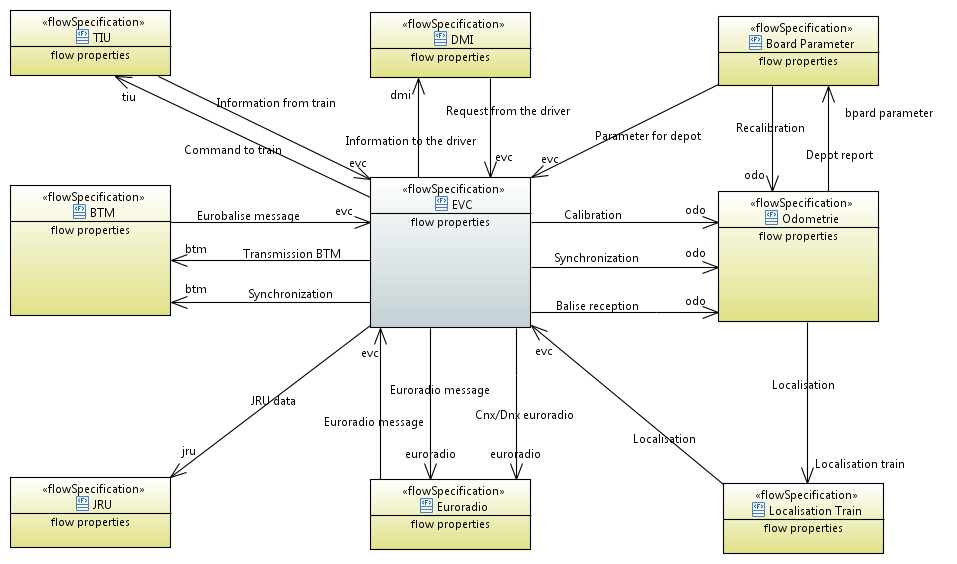
\includegraphics[scale=0.8] {images/HighLevelArchitecture.png}
\caption{SRS architecture}
\end{figure}

\begin{figure}[hbtp]
\section{Functional Breakdown}
\centering
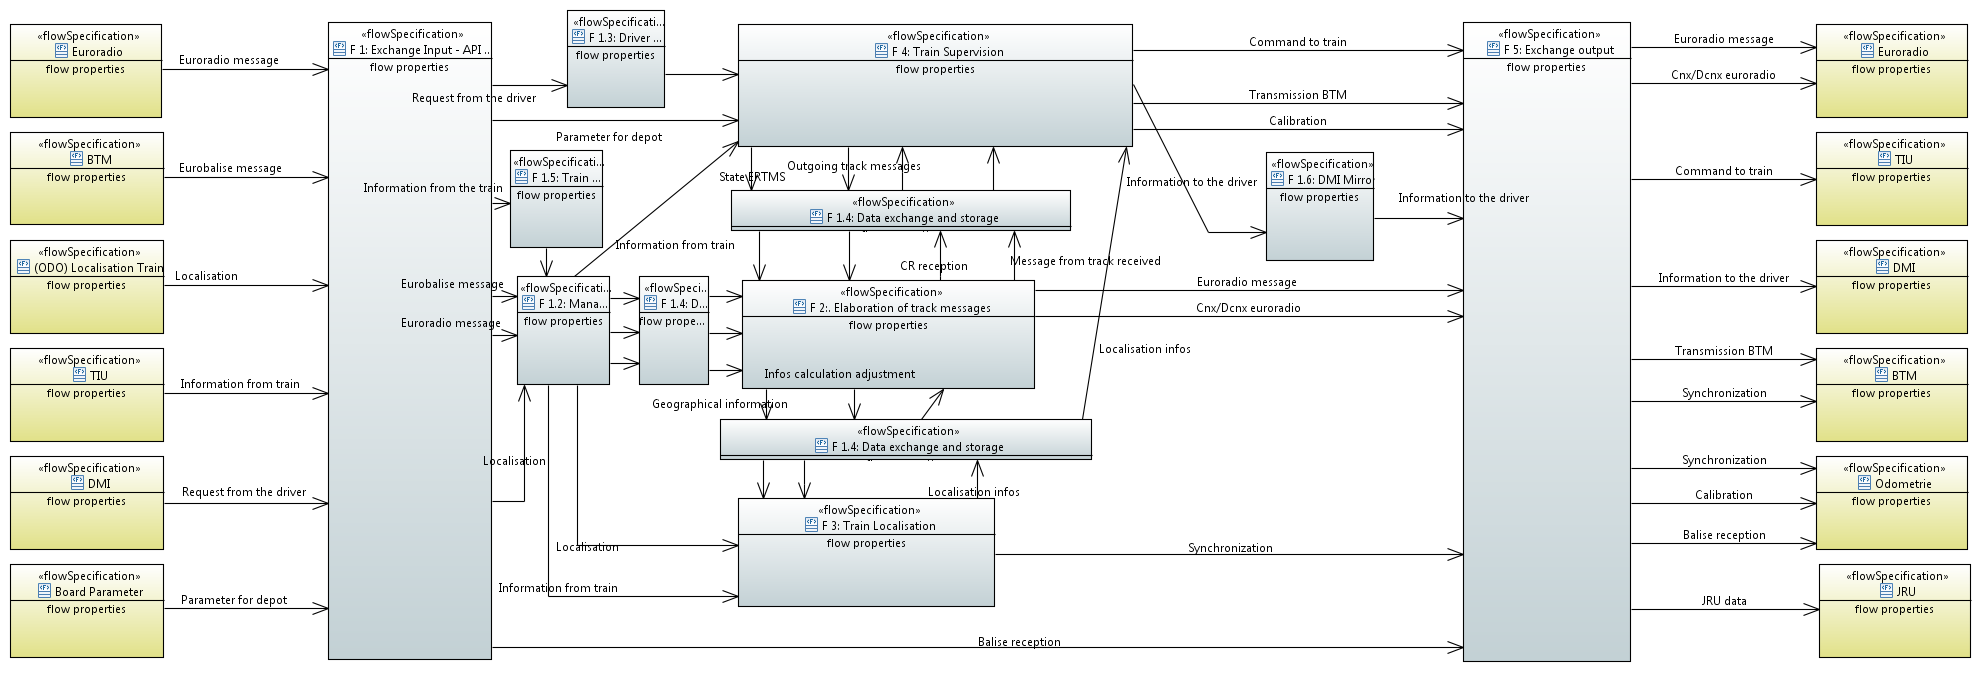
\includegraphics [angle=90, scale=0.5] {images/HighLevelFunctionalbreakdown}
\caption{SRS Breakdown}
\end{figure}

\newpage
\section{Description of the SRS Functions}

 \subsection{F1 Exchange input}

\textbf{See Figure 2 - Block F 1}\\
 
 Inputs:\\
``will be complete''\\
 
 Outputs:\\
 ``will be complete''\\
 
 Description: 
 This function module manages the interaction with the functional modules at the input and output 
of equipment: \\
- TIU, \\
- DMI, \\
- BTM, \\
- EURORADIO, \\
- Parameterization board, \\
- Displacement measurement.\\ 

It complements their functionalities at the level: 
the protocols and exchange "safety layer" with the kernel external modules, with 
Exception of Wegmessungsmoduls (this manages its own exchange protocols.
The summary of telepowering telegrams of the BTM module in a complete Eurobalise message a balise group with the same ID, with review of the 
Balisentelegramheader, management of the duplicated beacons and detecting the direction. 
In addition, the receipt of a Referenzbalise from the linked type, in addition to the 
Balise group, reported for the computational comparison of path measure modul. \\

 \subsection{F2 Elaboration track messages}
 
 \textbf{See Figure 2 - Block F 2}\\
 
  Inputs:\\
``will be complete''\\

 Outputs:\\
 ``will be complete''\\
 
 Description: This function module provides the encoding and decoding of track messages that 
Management of the port and power off RBC, and the management of reference 
Beacons, which are based on the track messages.\\

 \subsubsection{	F21: Receive Eurobalise Messages} 
 \textbf{SRS:} § 3.4, § 3.6, § 3.16, § 3.17, § 4.8\\
 
  \textbf{Inputs:}\\
``will be complete''\\

 \textbf{Outputs:}\\
 ``will be complete''\\
 
 \textbf{Description:} 
 This function module provides the summary of telepowering information and the 
review of coherence the content of telepowering message. 
This module separates the eurobalise message as follows: 
 
 - The Balise telegram heads for checking the consistency of the different 
Telegrams, the management of the duplicated beacons and the acquisition of meaning. \\

- Then the information that the balise group, their reading direction and are 
Wegmessungsposition where the first balise group was read, in 
Baliseninformationen for monitoring the function "Manage the eurobalises" 
summarized (see the term Identifzierung and meaning in this function), which the 
Continuation of reading via the information Referenzbalise with a Balisenposition in 
Kernel-reference document approved. \\

\textbf{- The ETCS ETCS version and packages:} \\

The first review is the version ETCS ETCS track with the version Zugbord 
(Version 1.x Class1 =) to compare; these must be compatible (that means 1.y) to 
continue processing (a Balise version of the type is 0.y as incompatible 
considered, but they must not generate a negative reception report). \\

The second review is in compliance with the ETCS grammar in the resulting 
Packets with a packet 255, which terminates the beacon information of each of the group. \\

The reception of a packet 245 (standard package) in a eurobalise) includes the 
Rejection of all other packets received and generated a the same mistake as 
Grammatical errors ETCS, unless the OBU is in Level 2. \\

Only the packets 44, 65, 66 and 136 may be located several times in a same eurobalise message\\ 
For the 136 package: \\
• a single packet 136 per Balise telegram, \\
• the different packages 136 in a same message are identical. \\

The read packets are filtered as a function: \\

- from the direction of the transition to the balise group (the packet is the variable 
QDIR oriented), 
the bi-default state (level, level of announced and ERTMS / ETCS mode). \\

The tables of filtering per level and ERTMS / ETCS mode are in the description of the 
Function "received EUR radio messages" contain.\\

\textbf{These packets are transmitted in four different groups:}

- Geographical information (packet 79 for the "train locations") \\

- Information CNX / DCNX (packets 42, 131) for the "the CNX and DCNX 
Euro Radio Management "\\

- Information Balise (package 136: Referenzbalise for in-fill information) for the function 
"Manage eurobalises" \\

- Track-mail received (other packages) for the "monitor train". \\

\textbf{Any error of Referenzbalise, the version or the grammar ETCS is in CR (radio channel) 
Receiving reported.}\\
 
 
 \subsubsection{F22: Receive Euroradio Messages}
  \textbf{SRS} § 3.4, § 3.6, § 3.16, § 4.8\\
  
    \textbf{Inputs:}\\
``will be complete''\\

 \textbf{Outputs:}\\
 ``will be complete''\\
 
\textbf{Description:} 
This function module provides the summary of the Euro radio information and the 
Verify the consistency of the contents of the Euro radio message. 
The first guaranteed by this module check is to monitor the radio link. 
This only applies to a normal communication channel (see § 8.3.1 interface gSM-R). \\

\textbf{The review is broken down as follows:}

- Basic principle: the RBC is providing its messages with a time stamp based on the 
Time marking the bi-standard the equipment (if the timestamp of the messages on 
position is undefined, the message is accepted, but only during the initialization of the 
Communication session EVC - RBC).\\

Verification of the sequence: \\

- the ETCS OBU train equipment rejects any message that is "older" than the last 
received message.\\

- the ETCS OBU train equipment is up to any message that is "younger" than the last 
received message.\\
 	 
 	 
\subsubsection{F23: Manage Eurobalise Messages}
\textbf{SRS} § 3.4, § 3.6, § 3.16\\
  
   \textbf{Inputs:}\\
``will be complete''\\

 \textbf{Outputs:}\\
 ``will be complete''\\
 
\textbf{Description:} 
This function module manages the Balise reference document of the Bi-Standard-train equipment, 
is said to know that the information supplied by the track following terms have: \\

- either the balise which provides the information, \\

- or delivered in the radio message Referenzbalise, \\

- or delivered in the infill balise message Referenzbalise (package 136). \\

A balise group contains 1-8 eurobalises. 
The balise group is referenced by an identification NIDLRBG (NIDC: identification 
+ NIDBG region: identification beacon). Each eurobalise has an internal number from 1 to 8, 
which describes the position of the beacon relaltive in the group. \\

A consisting of only one beacon balise group called "simple beacon", as 
any other balise group managed; However, it produces features that described in
Function module F23 and in the function module F25.\\

\subsubsection{F24: Manage Cnx and Dncx Euroradio}
\textbf{SRS} § 3.5, § 3.15.1, § 5.15\\

 \textbf{Inputs:}\\
``will be complete''\\

 \textbf{Outputs:}\\
 ``will be complete''\\
 
\textbf{Description:} 
This function module ensures the production ending a Euroradio- 
Communication. \\
For the ETCS OBU equipment it is possible to Euro Radio communication session
initiate: \\

- for a "start of mission": train data \\

- after one obtained from the track command: info CNX / DCNX. 
The command, an RBC to contact, the identity of the RBC and its telephone number 
(Packets 42 or 131).\\



 \subsubsection{F25: Send Euroradio Messages}
 \textbf{§ 3.4, § 3.16}\\
 
  \textbf{Inputs:}\\
``will be complete''\\

 \textbf{Outputs:}\\
 ``will be complete''\\
 
\textbf{Description:} 

This function module ensures the completeness (location and time stamp) and the 
Transmission of radio messages euro on the basis of information "radio session message", 
"Outgoing track message", "message acknowledgment" (for a radio message 136) and "CR 
Radio channel reception "(for a radio message 136 along with a package 4). \\

A radio message is sent only if between the Bi-Standard-board equipment and the 
RBC opened a euro radio session. \\

The radio messages, with the exception of the message confirmation (radio message 146) and the 
Session messages (radio message 154, 155, 156, 159) contain a "position report" package 
(O or 1 packet). \\

The structure of this "position report" package based on the following information: \\

- Info for locating the data LRBG, position, velocity, position error, moving direction,
Bi-default state for the data concerning the level and the ERTMS / ETCS mode. \\

The package 1 "special position report" is used for one or two LRBG whose 
Crossing direction is not known ((LRBG type simple balise group). \\

The package 0 "position report" is used when the direction of the LRBG is known (group 
not simple beacons, or group simple beacons, whose Balisenrichtung over by the track 
was positioned a link or package 135) (see function F23)).\\
 	
 \textbf{See the functional breakdown of the function in F2 in the next paragraph (Figure 3)}\\
 
\subsubsection{F2 breakdown}	
 \begin{figure}[hbtp]
\centering
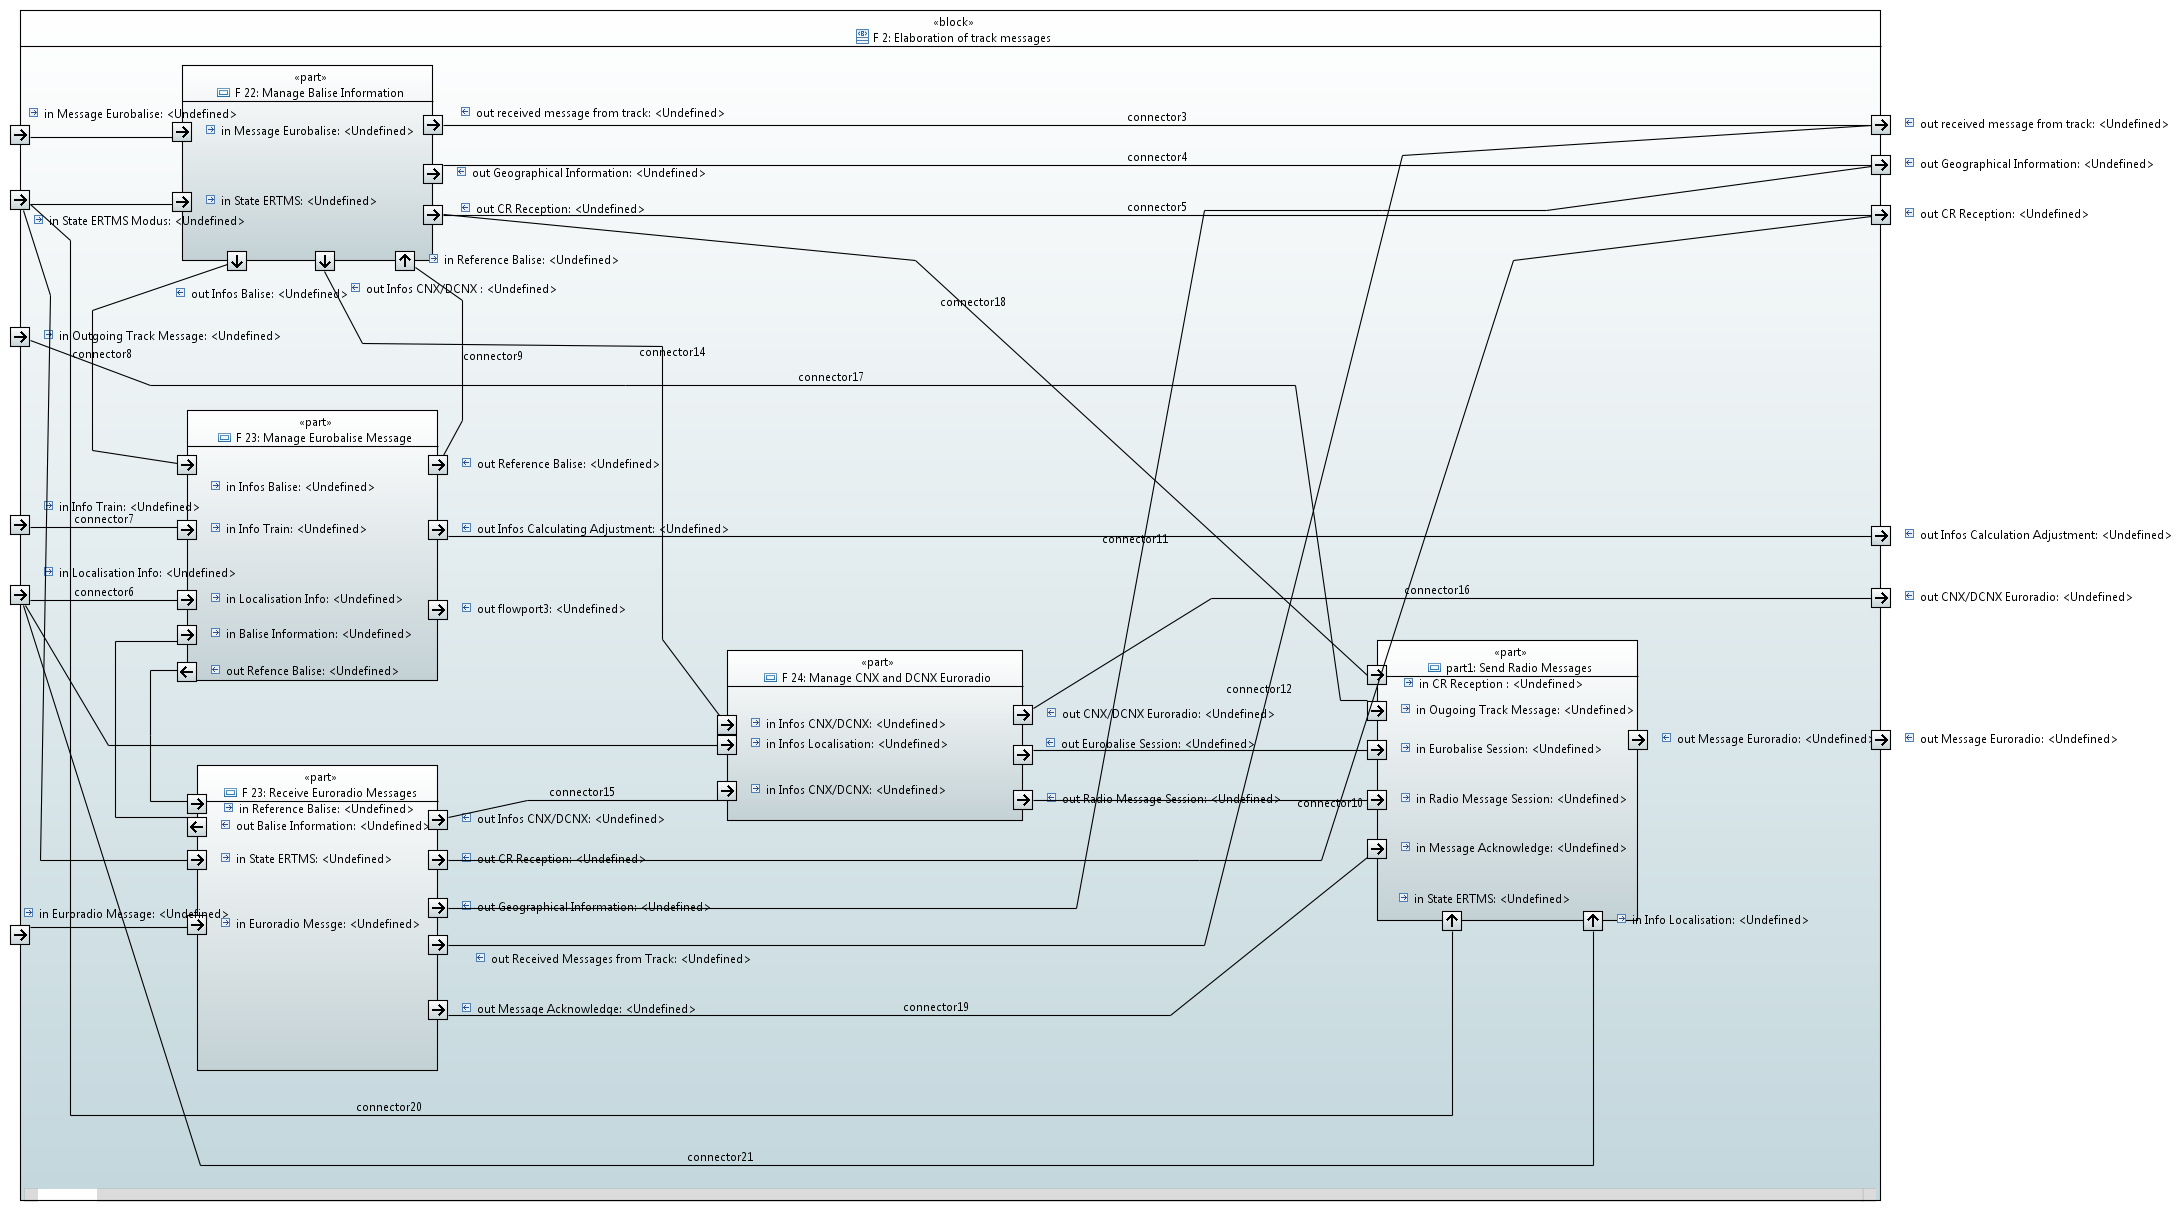
\includegraphics [angle=90, scale=0.4] {images/F2_Breakdown}
\caption{Elaboration track messages breakdown}
\end{figure}

\newpage
\subsection{F3 Train loction}
\textbf{See Figure 2 - Block F 3}\\

\textbf{SRS § 3.6.4, § 3.6.5, 3.6.6}\\

  \textbf{Inputs:}\\
``will be complete''\\

 \textbf{Outputs:}\\
 ``will be complete''\\
 
\textbf{Description:} 
This function module provides the location of the train in a kernel-reference document 
(Locating information), based on the following reference documents: \\

- path measurement calculation reference documents the function "distance measurement": train location, \\

- Balise the "track messages draw": Information computational comparison.\\


 \subsection{F 4 Train Supervising in ERTMS Modus}
F4: Train supervision in ERTMS Modus\\
F41: Manage Level ERTMS/ETCS SRS § 5.1, § 3.6.5\\
F42: Manage Modus ERTMS/ETCS § 4, § 3.6.5, § 3.15.4, § 5.5, § 5.6, § 5.7, § 5.9, § 5.11, § 5.13\\
F43: Train Speed supervision SRS § 3.7, § 3.8, § 3.10, § 3.11, § 3.12, § 3.13, § 5.7, § 5.8, § 5.9\\
F44: Train Movement supervision § 3.14\\
F45: Train position supervision § 3.6.5, 4.4.8, § 4.4.11\\
F46: Data storage (§ 4.3), § 3.18\\
F47: Dialog with the driver § 5.4, § 3.12.3\\
F48: Manage brake controll § 3.14.1\\ 
F49: Manage Train Controll, § 3.12.1\\
See Figure 4 - Block 4

 \subsection{F4 breakdown}	
 \begin{figure}[hbtp]
\section{F4 Functional Breakdown}
\centering
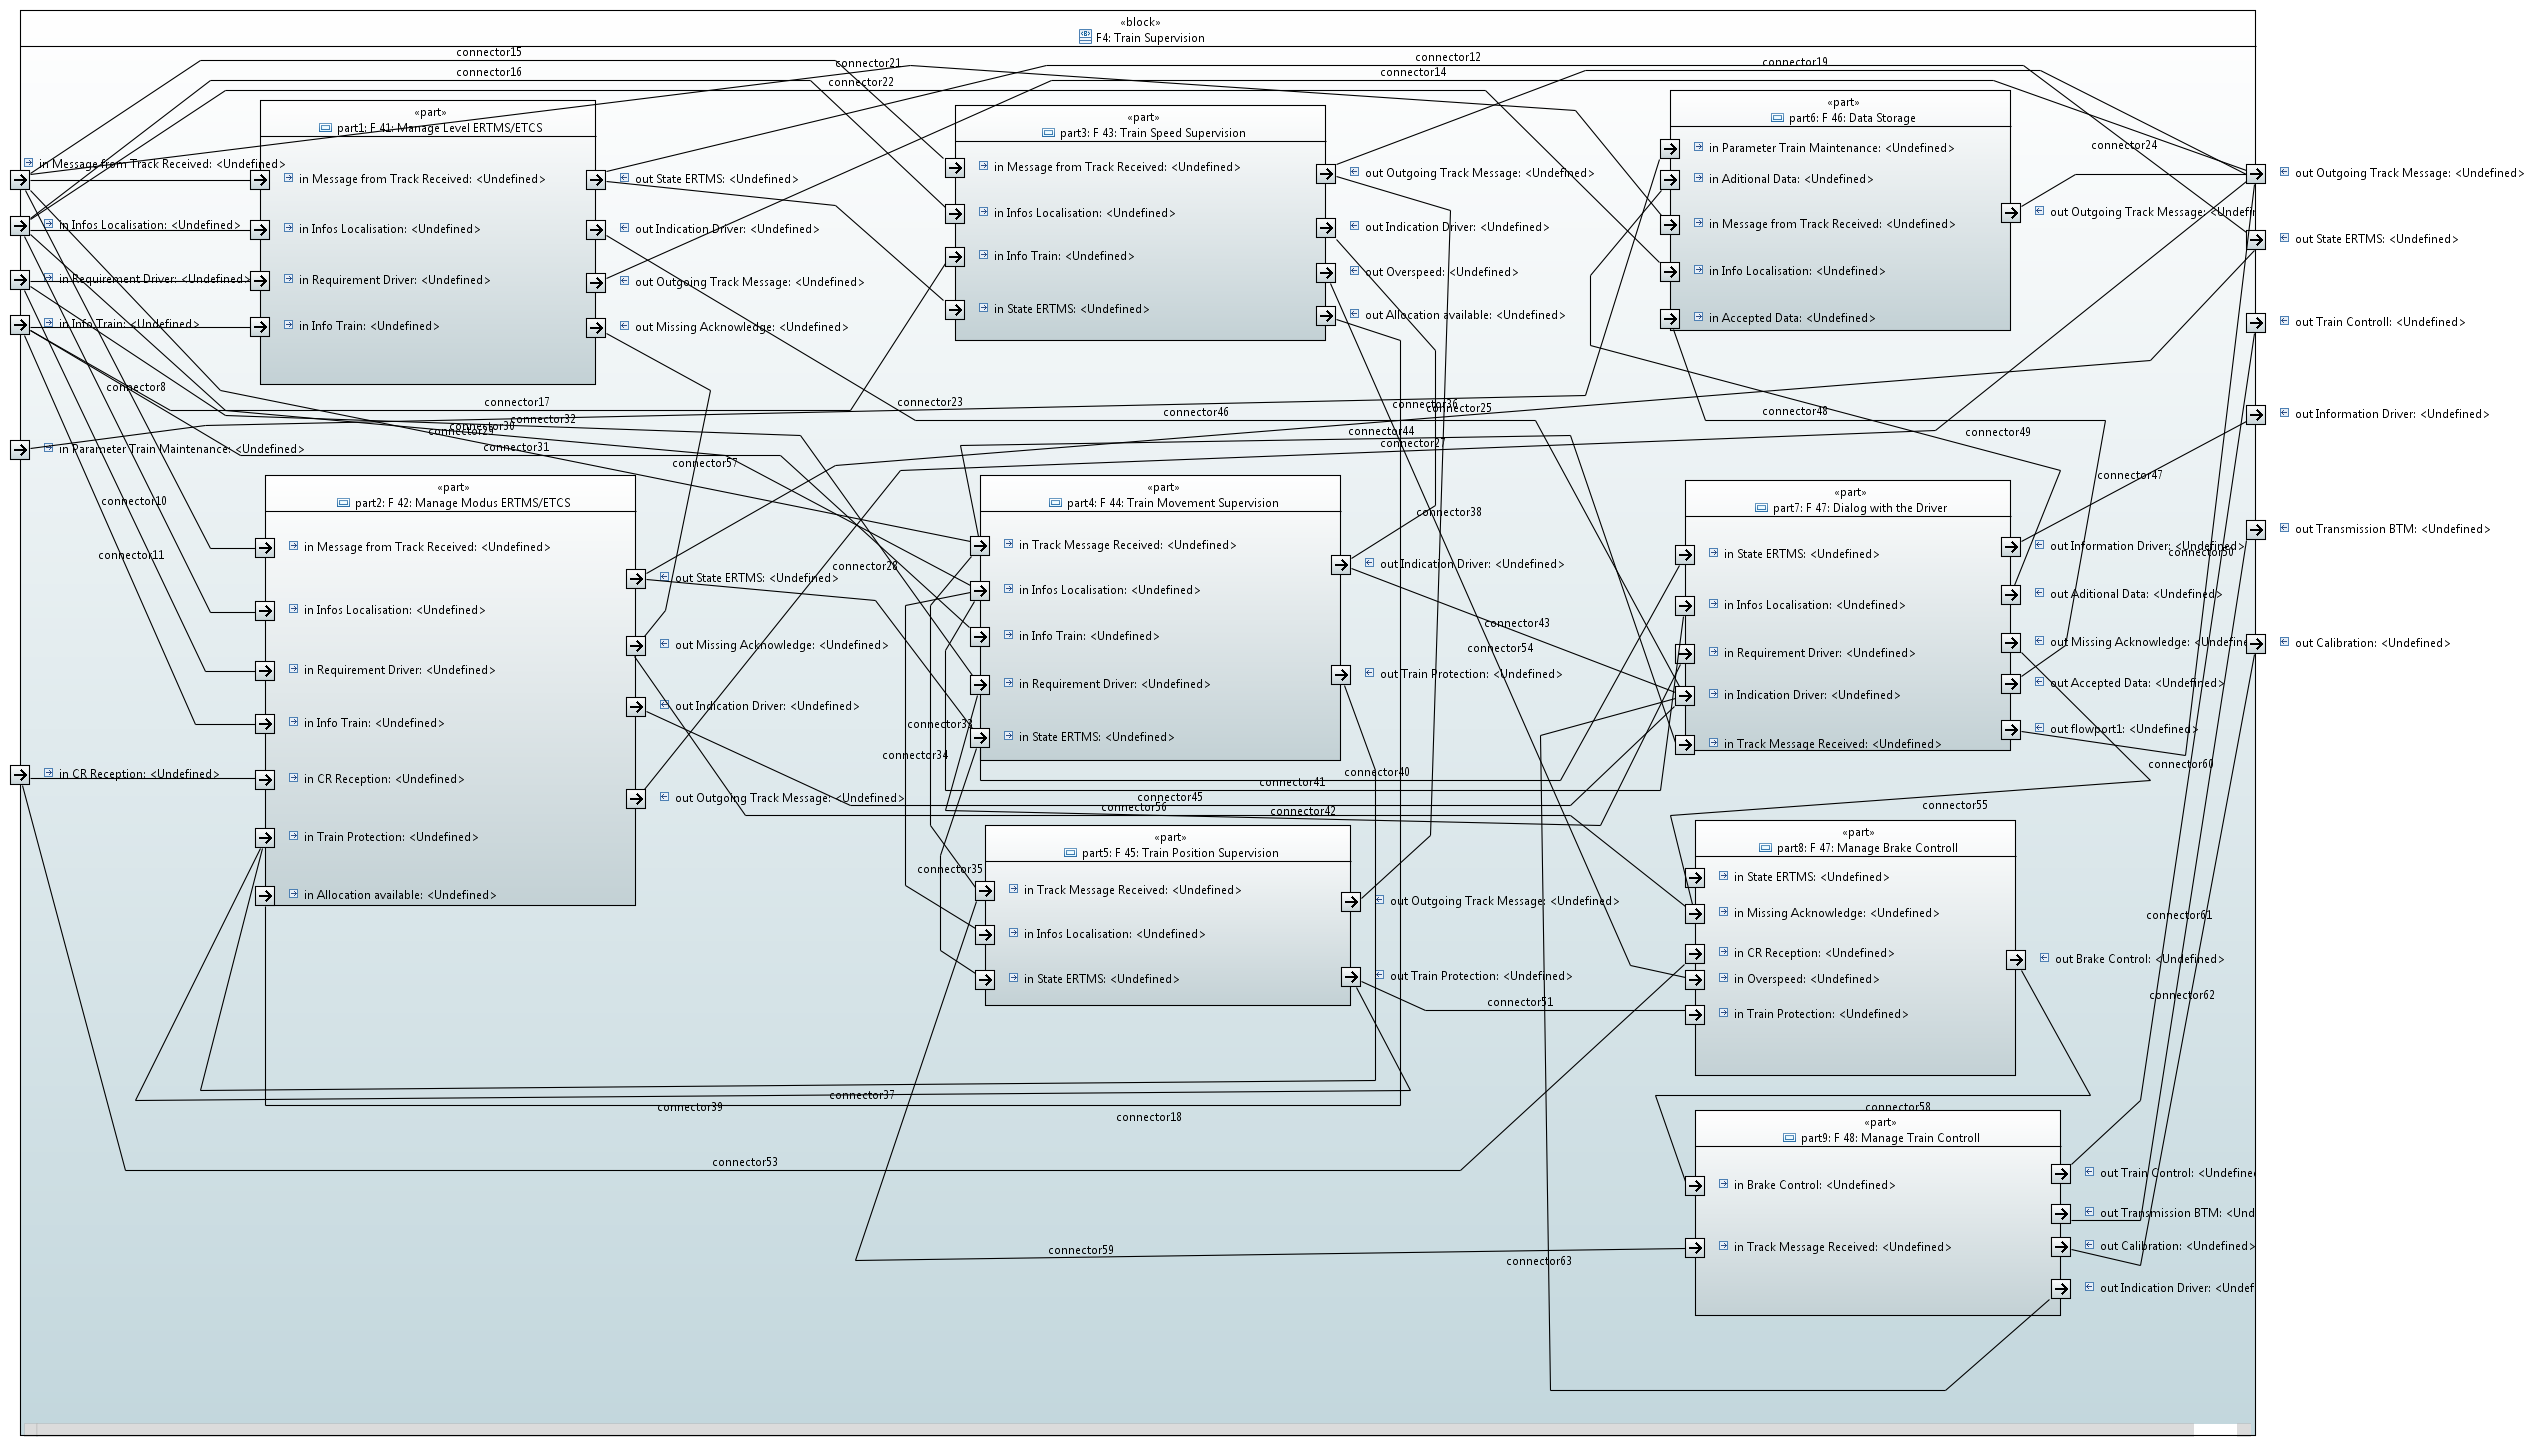
\includegraphics [angle=90, scale=0.35] {images/F4_Breakdown}
\caption{Train Supervising in ERTMS Modus}
\end{figure}

\newpage

 \subsection{F5 Exchange outpout}
 F5: Exchange output\\
 See Figure 2 - Block F 5\\
 
\subsection{Data Flow Description}
\tablefirsthead{
\hline 
\rowcolor{gray} 
Number & Flow & Source/Sink & Description  \\\hline}
\begin{supertabular}{| m{3,5cm} | m{3,5cm} | m{3,5cm} | m{3,5cm} |}
1.0 & Missing Acknowledge & Kernel xx/Kernel xx & This information indicates the absence of the 
Acknowledgment of the driver to a 
confirmatory text message on the Level 
Transition, the transition mode or a track 
Train-text message\\\hline
2.0 & Acknowledge & Kernel xx/Kernel xx & Radio message 146 transmission Confirmation - Confirmation message depending on the variable 
§ 8.6.7  \\\hline
3.0 & Action Driver & Kernel xx/Kernel xx &  Election / confirmation / detection Driver via DMI \\\hline
4.0 & Display Driver & Kernel xx/Kernel xx & For the driver specific DMI display \\\hline
5.0 & Reference Balise & Kernel xx/Kernel xx & information; in the Flow "information Balise"  delivered Balise confirmed as a reference beacon.\\\hline
6.0 & Allocation available & Kernel xx/Kernel xx & Information message that an allocation for a given technical mode is available.\\\hline
7.0 & Calibration & Kernel xx/Kernel xx & Specifying a calibration range of the 
path measurement.\\\hline
8.0 & Cnx/Dcnx Euroradio & Kernel xx/Kernel xx & Command on the connection and disconnection of a 
or of a RBC, the identity and 
Phone RBC contains.\\\hline
9.0 & Brake Controll & Kernel xx/Kernel xx & Control of the service and the 
emergency braking. \\\hline
10.0 & Train Controll (brake) & Kernel xx/Kernel xx & Functional output.\\\hline
11.0 & CR Reception (Radio Channel) & Kernel xx/Kernel xx & CR (radio channel) on receipt of a balise or 
Radio message: Checking version ETCS, 
Grammar ETCS, testing reference balise 
(Position), monitoring radio link\\\hline
12.0 & Accepted Data & Kernel xx/Kernel xx & Information valid confirmation of the train data and 
Consequently, at the very beginning of the mission.\\\hline
13.0 & Additional Data & Kernel xx/Kernel xx & Data relating to the mission of the train: 
Identity of the driver, 
selected level, identity and mandatory. of the RBC, 
if Level 2, no. Mission\\\hline
14.0 & JRU Data & Kernel xx/Kernel xx & Recorded legal data.\\\hline
15.0 & Input Train & Kernel xx/Kernel xx & From the train coming TOR digital inputs and 
Digital outputs \\\hline
16.0 & State ERTMS & Kernel xx/Kernel & Current Level and operating mode ERTMS, announced ERTMS Level and Current Level and operating mode ERTMS, announced ERTMS Level\\\hline
17.0 & Indication Driver & Kernel xx/Kernel xx & each specific for the driver 
Specification. This includes the dynamic information 
speed monitoring the 
different messages and symbols, the 
Exchange during the "start of mission"\\\hline
18.0 & Info Train & Kernel xx/Kernel xx & From Train comming functional information TIU \\\hline
19.0 & Message Eurobalise & Kernel xx/Kernel xx & Information, which the ID 
Balise group (country ID + ID 
Balise), their reading direction and their 
Contains path measurement for review 
(see Flow "reference balise")\\\hline
20.0 & Information cnx/dcnx & Kernel xx/Kernel xx & Information identifying the RBC ID 
(Identification of land + the identification of the RBC), 
RBC his phone number and the authorization \\\hline
21.0 & Information Driver & Kernel xx/Kernel xx & Specific for the driver 
Function DMI information. They contain the 
different specifications for the 
Driver, which are generated from the 
different Function modules.\\\hline
22.0 & Geographical information & Kernel xx/Kernel xx & Absolute current position of the train, which the 
add the flow "location information" \\\hline
23.0 & Information Localisation & Kernel xx/Kernel xx & Locating the train: position and speed of the train in the 
different reference documents, 
including the absolute geographical 
Position.\\\hline
24.0 & Message Eurobalise & Kernel xx/Kernel xx & Flow, summarizing the message / messages eurobalise. 
BTM to F1: the entire telegrams 
F1 to F2: Message 
(the safety layer and the 
the safety layer and the transfer of 
Telegrams in a message by F1 
F1 guaranteed)\\\hline
25.0 & Infos Calculation Adjustment & Kernel xx/Kernel xx & Information, which contains the ID 
Balise group (country ID + ID 
Balise), their path measurement and her for the 
computational comparison of the on-board 
Contains reference document expected position\\\hline
26.0 & Localisation Train (ODO) & Kernel xx/Kernel xx & path measurement in comparison to a 
Balise (+ safety margin), Speed ​​(+ 
Safety distance), direction of travel and capture 
of stopping\\\hline
27.0 & Euroradio Message (train to track) & Kernel xx/Kernel xx & Transmitted Euro radio message 
(the safety layer is guaranteed by F5)\\\hline
28.0 & Euroradio Message (track to train) & Kernel xx/Kernel xx & Received Euro radio message 
(the safety layer is guaranteed by F1)\\\hline
29.0 & Radio Message Session & Kernel xx/Kernel xx & Message / parcel Euro Radio for creating and 
Termination of the radio connection\\\hline
30.0 & Outgoing Track Message & Kernel xx/Kernel xx & Before Inform creation and timestamp 
(except the message flow 
Radio link, message confirmation and CR 
Reception) sent to the track to 
function message\\\hline
31.0 & Message from Track Received & Kernel xx/Kernel xx & Via radio or beacon message received function 
(except the Riverside current 
Information, cnx / dcnx information, Balise 
information)\\\hline
32.0 & Parameter Train maintenance & Kernel xx/Kernel xx & Fixed data, train data, domestic values\\\hline
33.0 & Train Protection & Kernel xx/Kernel xx & Information, protection against rolling 
Twitching, monitoring of stopping, the 
Transition to an unauthorized Balise in SH 
or SR reports\\\hline
34.0 & Balise Reception & Kernel xx/Kernel xx & Information of receipt of a reference Balise NPIG = 0 from the associated type for the computational comparison of the displacement measurement\\\hline
35.0 & Requirement Driver & Kernel xx/Kernel xx & By driver outbound (see flow 
"Action Driver") or from DMI DMI produced 
function information\\\hline
36.0 & Euroradio Session & Kernel xx/Kernel xx & State of the Euroradio connection \\\hline
37.0 & Signal Eurobalise & Kernel xx/Kernel xx & Airgap Eurbalise -> BTM\\\hline
38.0 & Signal Euroradio & Kernel xx/Kernel xx & Airgab RBC ->Euroradio Board\\\hline
39.0 & Output Train & Kernel xx/Kernel xx & Train digital outuputs\\\hline
40.0 & Overspeed & Kernel xx/Kernel xx & Information message overspeed
of the train relative to the
speed curves\\\hline
41.0 & Synchronization & Kernel xx/Kernel xx & Synchronization (xw, V, T) between the kernel, 
the BTM and the path measurement\\\hline
42.0 & Transmission BTM & Kernel xx/Kernel xx & Control BTM - antenna\\\hline
\end{supertabular}
 
 \subsection{current partly openETCS Architecture}
 Needs to be integrated into the overall architecture .....
  \begin{figure}[hbtp]
\centering
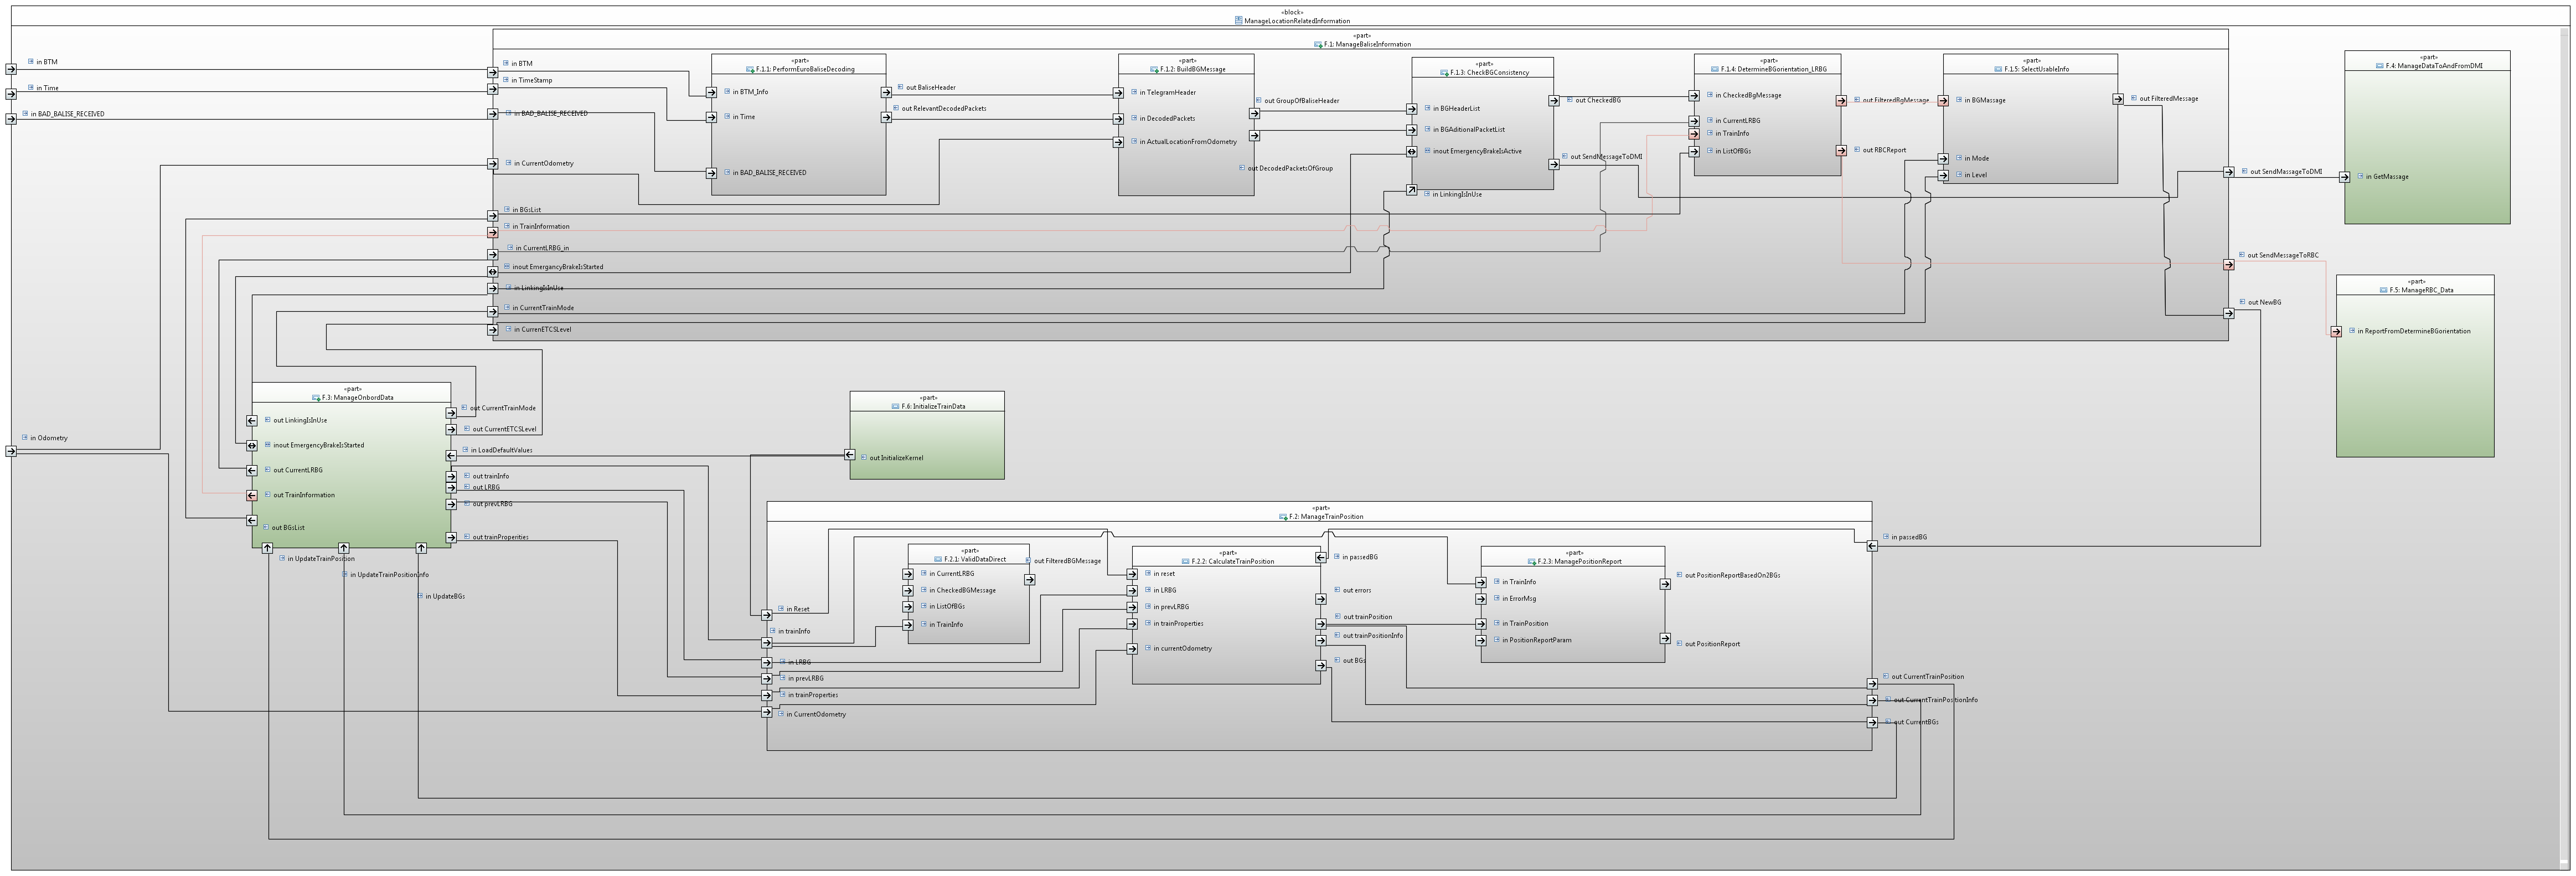
\includegraphics [angle=90, scale=0.2]{images/Current_partly_openETCS_architecture}
\caption{Centralized data structure approach architecture}
\end{figure}
 
 
 \newpage
 \subsection{centralized data structure approach}
 \begin{figure}[hbtp]
\centering
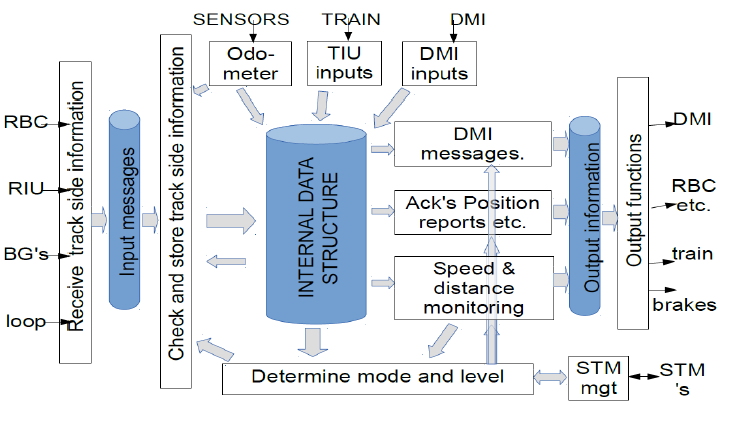
\includegraphics [scale=0.6] {images/CentralizedDataStrukture_2}
\caption{Centralized data structure approach architecture}
\end{figure}


 \begin{figure}[hbtp]
\centering
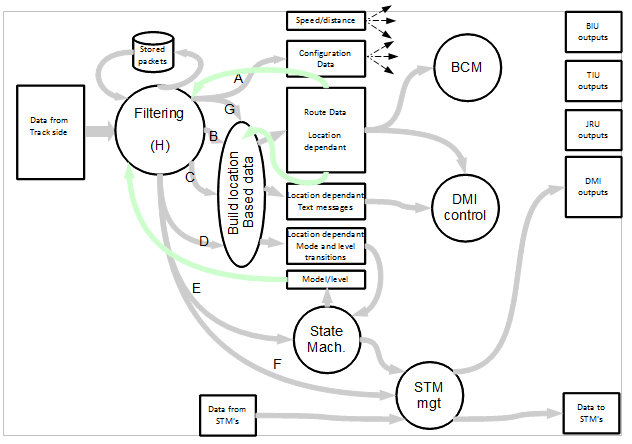
\includegraphics [scale=0.7] {images/CentralizedDataStructure_1}
\caption{Centralized data structure approach breakdown}
\end{figure}

\newpage

\subsection{Alstom High Level Approach}
 \begin{figure}[hbtp]
\section{Alstom High Level SRS Architecture}
\centering
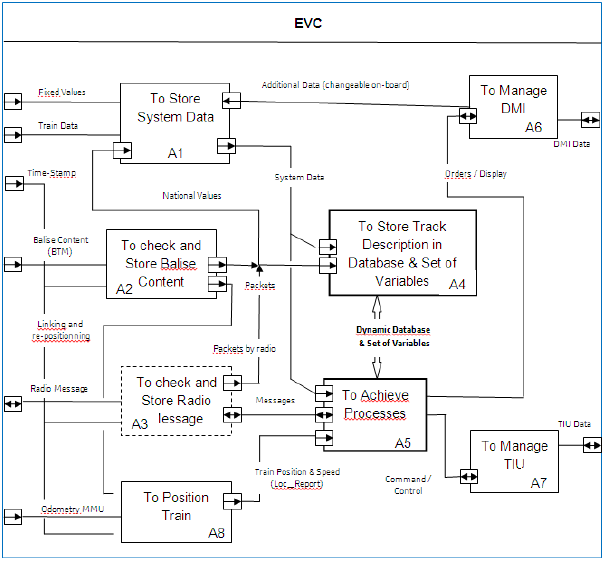
\includegraphics [scale=0.8] {images/Alstom_High_Level_Approach}
\caption{Alstom SRS Architecture Approach}
\end{figure}

\newpage
\subsection{The openETCS Tool-Chain and its impacts on the actual model}

For understanding the modelling process and the modeling guidelines, we refer to \url{https://github.com/openETCS/modeling/blob/master/DescriptionOfWork/NewModelingDescriptionOfWork.pdf}.

To summarize the design process, the following rules are in use:
\begin{itemize}
\item Papyrus / SysML is used for modelling the architecture. Functions are visible on this SysML level.
\item No behaviour model is allowed on SysML level.
\item For referencing the requirements, links from the SysML model to the requirements document (in ProR) are being used.
\item Details and especially behaviour is part of the Scade models.
\item All interfaces (see also data-dictionary below) are available on bit-level.
\item In the architecture model in SysML, all interfaces are available on a functional level for interfaces inside and outside the model and for interfaces between dedicated functions. Due to tool constrains the current model does not show all details for all interfaces (see dataDictionary).
\end{itemize}

The openETCS tool-chain for doing the modelling work consists of the following components:
\begin{itemize}
	\item [\textbf{Papyrus}]: for modelling the architecture (Kepler version).\\
	In this phase only the Kepler version of the tool can be used due to incompatibilities of the Kepler and the Luna version on the SysML model. The SysML models are stored in the following location: \url{https://github.com/openETCS/modeling/tree/master/model/sysml}.
	\item [\textbf{ProR}]: for keeping the requirements (REQIF).\\
	The subset 26 is converted into a REQIF-format and also stored in the modeling repository on Github. The openETCS toolchain supports the linking of SysML model parts to SRS-Requirements. These results are also part of the architecture.
	\item [\textbf{Scade}]: for designing and formalising the functions Scade version 15.2 is used.\\
	The models are stored in this location: \url{https://github.com/openETCS/modeling/tree/master/model/Scade}.
	With the component Scade System Scade also has a component for designing the architecture.
\end{itemize}

In principle, the synchronisation mechanism of Scade was planned to be used for synchronising the SysML architecture and the Scade models. The idea is to automatically synchronise the SysML types and blocks with the Scade type definitions and the Scade Operators. Unfortunately, with the current set of tools this idea cannot be realised. We will investigate other tools and models to find a solution. 

In addition, faults in the Kepler Papyrus version made it difficult for several members of the team to work on different submodels of the openETCS model. The issue will be solved when changing to the Luna version of Papyrus.



\section{Functions of the openETCS Model}

\subsection{openETCS Data Dictionary}

/subsubsection{dataDictionary}
%Peyman

\subsection{openETCS Generic API}


The openETCS system contains two APIs (Application Programming
Interface):
\begin{enumerate}
\item \emph{openETCS API}: the interface specification between the
EVC platform and the openETCS application;
\item \emph{model API}: the interface between the model itself written in
SCADE and the surounding run-time. Both the SCADE model and the
run-time are making the openETCS application.
\end{enumerate}

\begin{figure}[h]
\centering
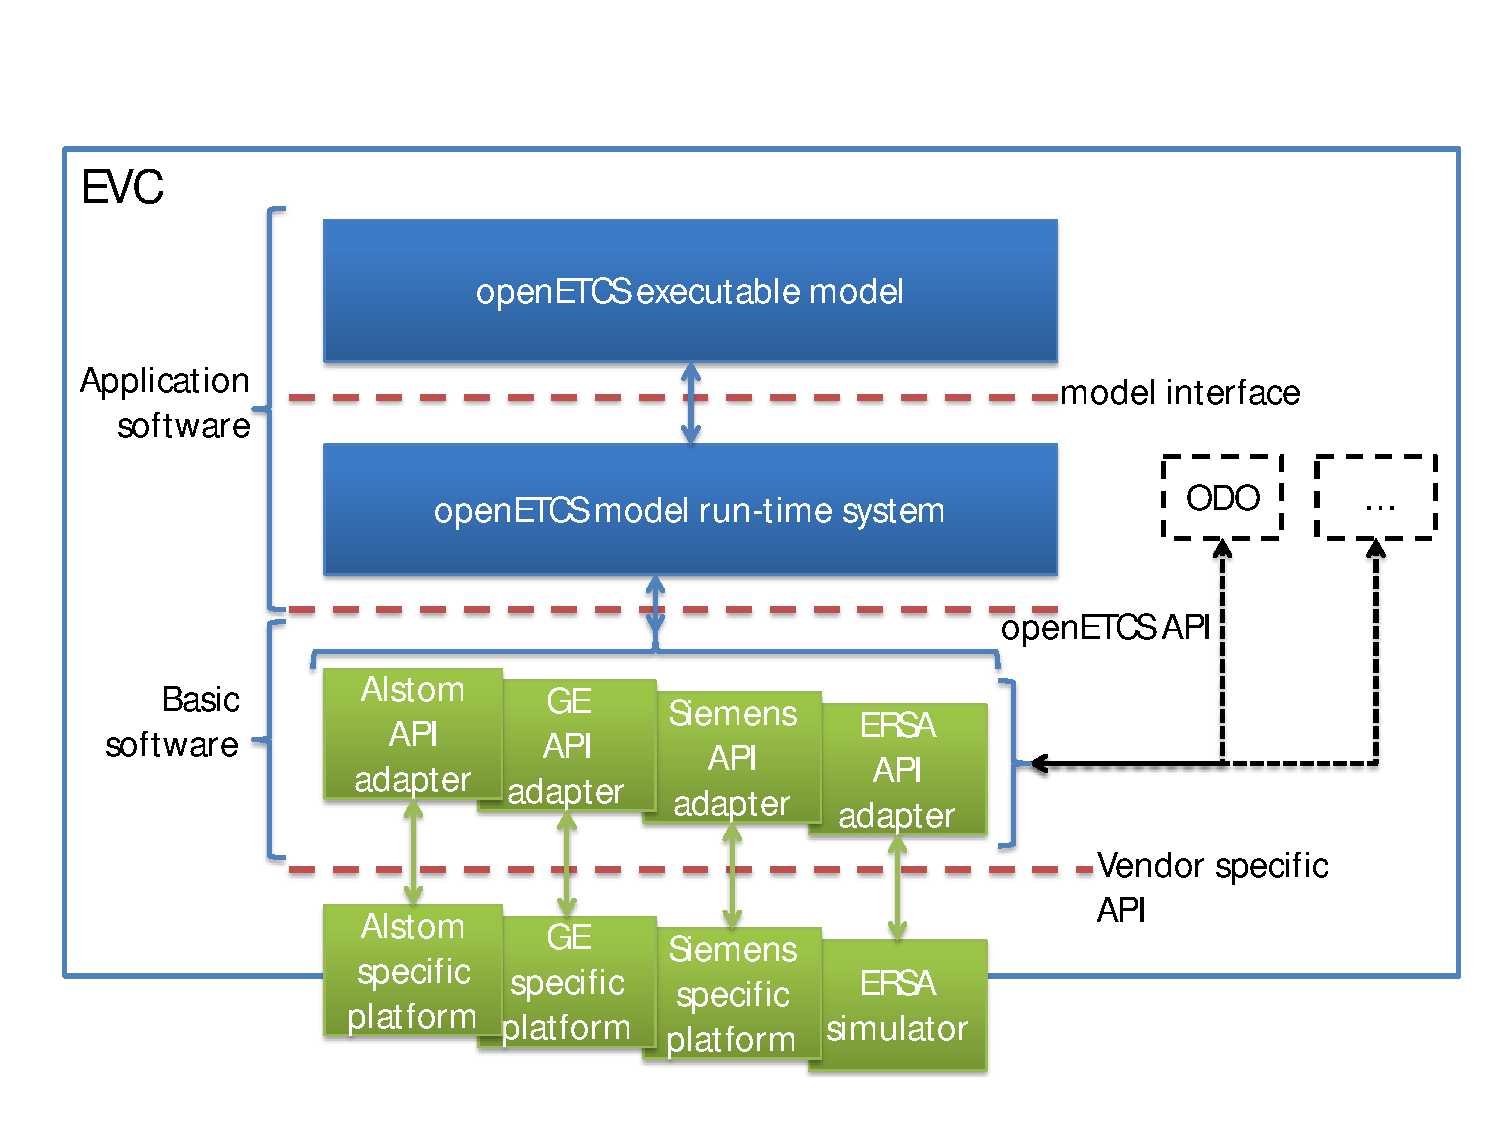
\includegraphics[width=\textwidth]{software-architecture.pdf}
\caption{openETCS software architecture}
\label{fig:software-architecture}
\end{figure}

Figure \ref{fig:software-architecture} shows both openETCS API and
model API on the software stack.

\subsubsection{openETCS API}

The openETCS API is currently defined by two documents, one written by
Alstom \cite{alstom-api} and a more abstract specification written by
openETCS members \cite{openetcs-api}.

The openETCS API defines the interfaces between the EVC platform and
the openETCS application for the following units surrounding the EVC:
\begin{itemize}
\item TIU (Train Interface Unit);
\item ODO (Odometry);
\item DMI (Driver Machine Interface);
\item STM (Specific Transmission Module, up to 8 units);
\item BTM (Balise Transmission Module);
\item LTM (Loop Transmission Module);
\item EURORADIO;
\item JRU (Juridical Recording Unit);
\item Zero or more Vendor specific unit.
\end{itemize}


\subsubsection{Model API}

The model API is currently defined by the inputs and outputs of the SCADE model.

\FIXME{How to give a precise pointer within the SCADE model? Reference
to a specific block within the model?}

For the proper working of the SCADE model, a set of assumptions are assumed:
\begin{itemize}
\item \textbf{Eurobalise (BTM)}: It is assumed that at most one
``telegram'' is provided per call of the SCADE model. This
``telegram'' is the merge of the telegrams of the balises making a
balise group.
\end{itemize}

% LocalWords:  SCADE API openETCS Alstom EVC EURORADIO Odometry balises balise


\subsection{openETCS Balise Group}


\subsubsection{Receive Eurobalise From API}
\begin{itemize}
\item \textbf{Short Description of Functionality}\\
This function defines the interface of the OBU model to the openETCS generic API for Eurobalise Messages. On the interface, either a valid telegram is provided or a telegram is indicated which could not be received correct when passing the balise. The function passes the telegram without major changes of the information to the next entity for collecting the balise group information.

%\item \textbf{{Reference to the SRS (or other requirements}\\
\item \textbf{Design Constrains and Choices}\\
\begin{enumerate}
\item Decoding of balises is done at the API. Also, packets received via the interface are already transformed into a usable shape.
\item Only packets used inside the current model are passed via the interface:\\
	Packet 5: Linking Information.\\
	Linking Information is filled into the linking array starting from index 0 without gaps. Used elements are marked as valid. Elements are sorted according to the order given by the telegram sequence.
\end{enumerate}
\end{itemize}


\subsubsection{Build BG Group}
\begin{itemize}
\item \textbf{Short Description of Functionality}\\
This entity collects telegrams received via the interface into Balise Group Information.
\item \textbf{Reference to the SRS (or other requirements}\\
\item \textbf{Design Constrains and Choices}\\
\begin{enumerate}
\item Telegrams received as invalid are passed to the ``Check-Function'' in order to process errors in communication with the trackside according to the requirements and in a single place.
Telegrams are filled into the telegram array starting from index 0 without gaps. Used elements are marked as valid. Elements are stored according to the order given by the telegram sequence. 
\item Only packets used inside the current model are passed via the interface:\\
	Packet 5: Linking Information.\\
\item In this function packets past with the telegrams is accumulated into a balise group information.\\
\item Further assumption on packet 5 (based on SRS subset 26, section 8.4.1.4)\\
(In this statement the term ``message'' is ambiguous since it can reflect to a telegram or a balise group message)
	Linking Information can only be passed once. This means, if linking information for the balise group is already collected with one of the earlier telegrams, the information will not be accumulated but overwritten.\\
\end{enumerate}
\end{itemize}

\subsubsection{Check BG Consistency}

\subsubsection{Determine BG- Orientation and LRBG}
\begin{itemize}
\item \textbf{Short Description of Functionality}\\
\item \textbf{Reference to the SRS (or other requirements}\\
\item \textbf{Design Constrains and Choices}\\
\end{itemize}
			
\subsubsection{Select Usable Info}


\subsubsection{Perform Balise Decoding}
\subsection{openETCS Train Position}

\subsubsection{F.2.2 Calculate Train Position}\label{sss:calctrainpos}

\begin{itemize}
\item \textbf{Short Description of Functionality}\\
The main purpose of the function is to calculate the locations of linked and unlinked balise groups (BGs) and the current train position while the train is running along the track. 

\begin{figure}[hbtp]
\centering
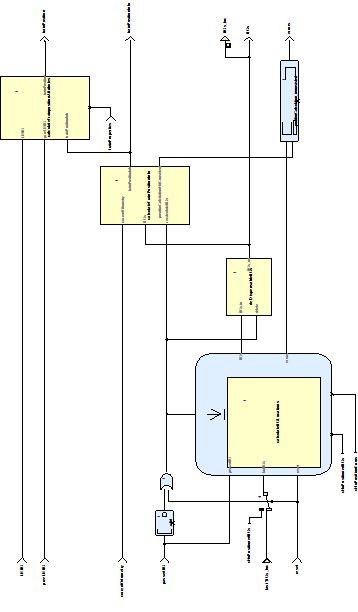
\includegraphics[scale=1]{../images/CalculateTrainPosition.png}
\caption{Structure of calculateTrainPosition}
\end{figure}


\paragraph{Functional Structure in Stages}
The whole function calculateTrainPosition is subdivided into the following steps, which are performed sequentially: 
\begin{enumerate}
\item \textbf{\textit{calculateBGLocations}}: Calculate the balise group locations\\
The first stage is triggered each time the train passes a balise group (input \textit{passedBG}). It takes the balise group header with the BG identification, the linking information (Subset 26, packet 5) and the current odometry values as inputs and calculates the location of the the passed balise group. If the passed BG has been announced via linking information previously, it takes into account the linking as well as the odometry information. If the passed BG does not meet the tolerance window announced by linking, an error flag is set. If the passed BG is an unlinked BG, its location is determined by odometry only, but related to the next previously passed linked BG, if there is one.\\
Then, if the passed BG is a linked BG comprising linking information for BGs ahead, the linking information is evaluated by creating the announced BGs and computing their locations from the linking distances.\\
The passed and the announced BGs are stored in a list \textit{BGs}, ordered by their nominal location on the track.\\
Afterwards the locations of all BGs are further improved by re-adjusting their locations with reference to the just passed BG. This optimizes the BG location inaccuries around the current train position (= location of the passed BG). 

\item \textbf{\textit{delDispensableBGs}}: Delete dispensable balise groups\\
The second stage removes balise groups supposed not to be needed any longer from the list of \textit{BGs}.\\
If the number of stored passed linked BGs exceeds the maximum number of eight as specified in subset-26-3.6.2.2.2 c), all BGs astern are deleted.
If only (passed) unlinked BGs are in the list and exceed the number of \textit{cNoOfAtLeast\_x\_unlinkedBGs}, all passed BGs astern to those are removed from the list. 

\item \textbf{\textit{calculateTrainPositionInfo}}: Calculate train position information.\\
This stage take the list of stored BGs and the current odometry values as inputs and steadily provides the current train position. 

\item \textbf{\textit{calculateTrainpositionAttributes}}: Calculate train position attribute information.\\
This stage provides several additional position related attributes that might conveniently be used by subsequent consumers in the architecture. It requires the actual LRBG and the previous LRBG to be assigned external from the list \textit{BGs}. 

\end{enumerate}

\item \textbf{Reference to the SRS (or other requirements)}\\
\\
The component calculateTrainPosition determines the location of linked and unlinked balise groups and the current train position during the train trip as specified mainly in subset-026-3.6

\item \textbf{Design Constraints and Choices}\\
\\
The following constraints and prerequisites apply:

\begin{enumerate}
\item The input data received from the balises groups must have been checked and filtered for validity, consistency and the appropriate train orientation before delivering them to calculateTrainPosition. 
\item The storage capacity for balise groups is finite. calculateTrainPosition will raise an error flag when a balise group cannot be stored due to capacity limitations.
\item calculateTrainPosition will raise an error flag if a just passed balise group is not found where announced by linking information. It will not (yet) detect when an announced balise group is missing. 
\item calculateTrainPosition is not yet prepared for train movement direction changes. 
\item calculateTrainPosition does not yet consider repositioning information.
\end{enumerate}

\end{itemize}

\subsubsection{Provide Position Report}\label{sss:provposrep}

\begin{figure}[ht]
\centering
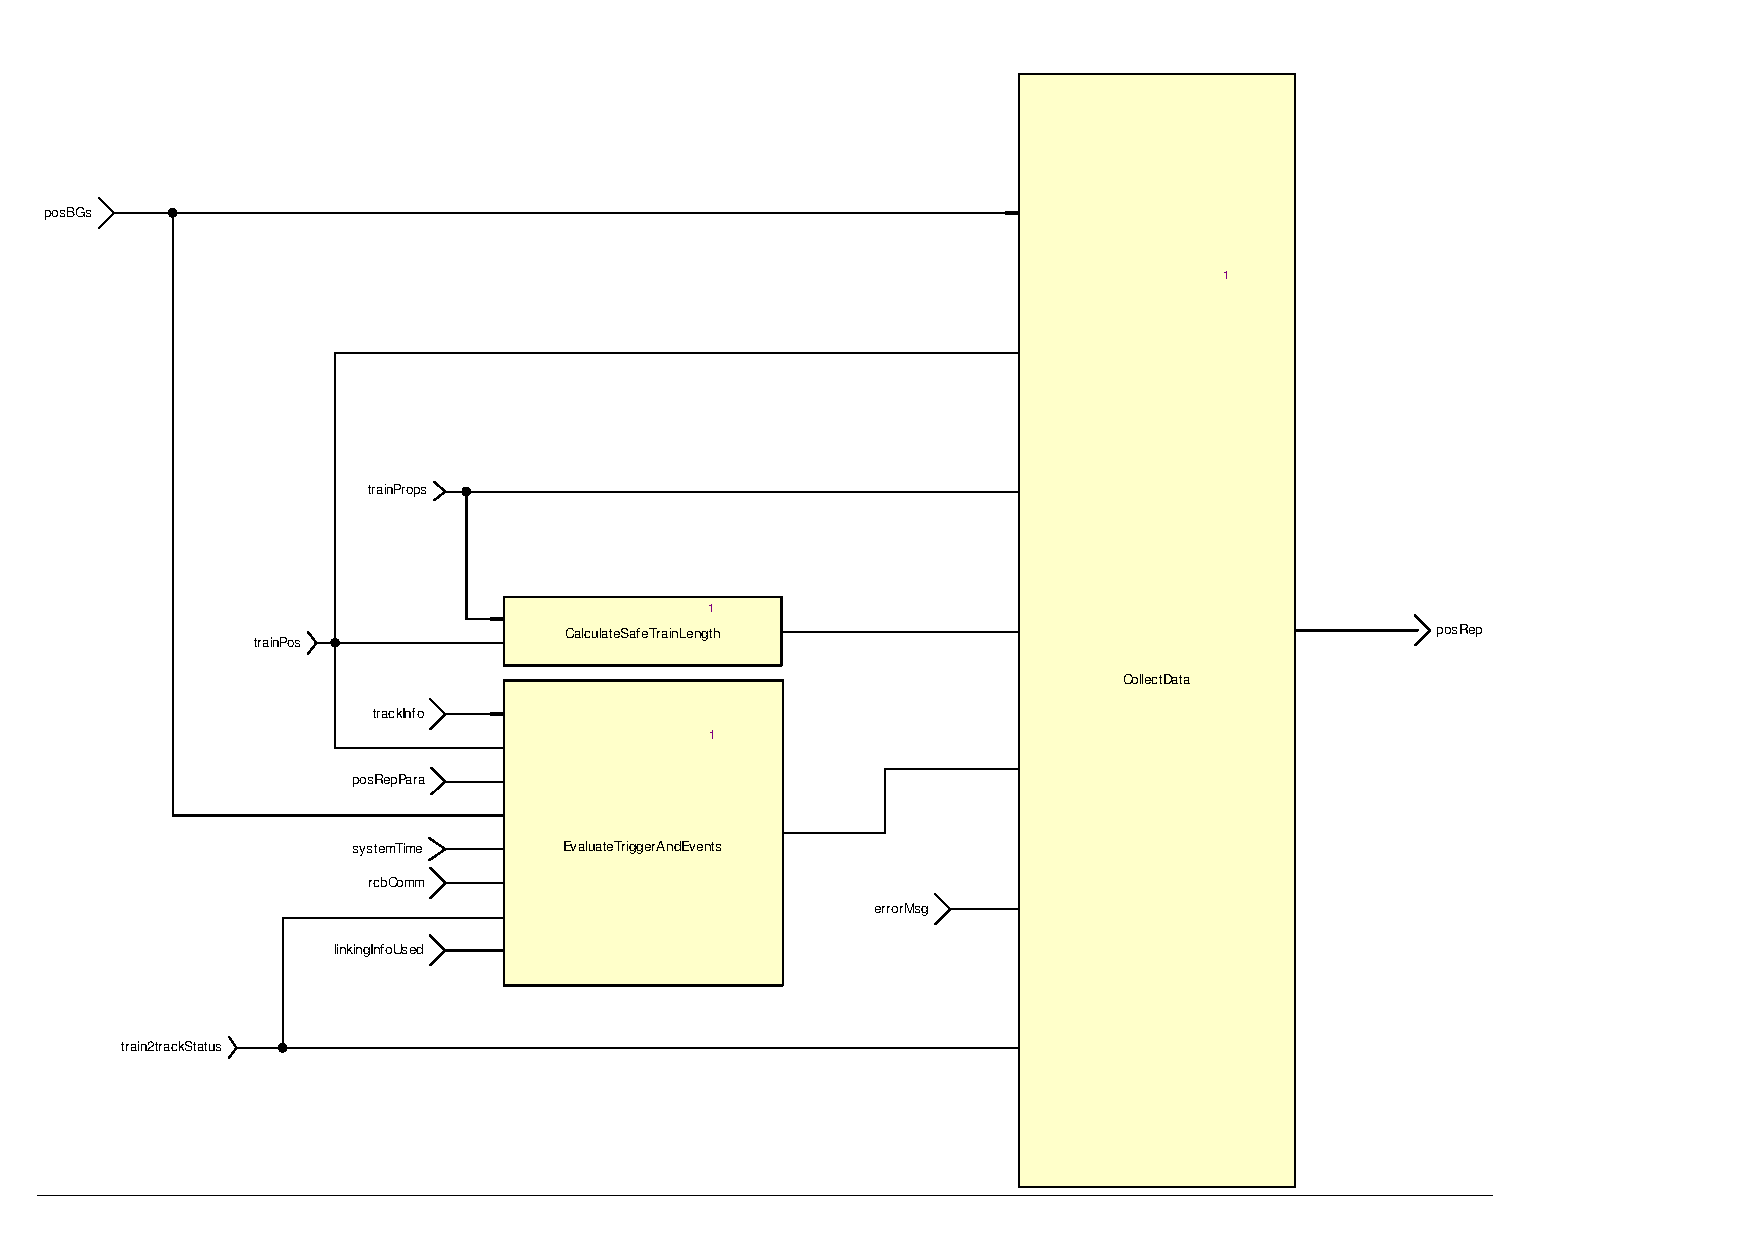
\includegraphics[scale=0.6]{../images/ProvidePositionReport.pdf}
\caption{Structure of component ProvidePositionReport}\label{fig:provideposrep}
\end{figure}

\begin{itemize}
\item \textbf{Short Description of Functionality}\\
This function takes the current train position and generates a position report which is sent to the RBC. The point in time when such a report is sent is determined from event, on the one hand, and position report parameters---which are basically triggers---provided by the RBC or a balise group passed, on the other hand. The functionality is modeled using three operations, as shown in Fig.~\ref{fig:provideposrep}, which are explained below.
\begin{description}
	\item[CalculateSafeTrainLength] Calculates the the safeTrainLength according to Chapt.~3.6.5.2.4/5.
\verb+safeTrainLength = absolute(EstimatedFrontEndPosition - MinSafeRearEnd)+, where
\verb+MinSafeRearEnd = minSafeFrontEndPosition - L_TRAIN+
	\item[EvaluateTriggerAndEvents] Returns a Boolean modeling whether the sending of the next position report is triggered or not. It is the conjunction of the evaluation of all triggers (PositionReportParameters, i.e., Packet 58) and events (see Chapt.~3.6.5.1.4).
	\item[CollectData] In this operation, data of Packet0, \dots, Packet5 and the header is aggregated to a position report.
\end{description}
\item \textbf{Reference to the SRS (or other requirements}\\
Most of the functionality is described in subset 26, chapter~3.6.5.
\item \textbf{Design Constrains and Choices}\\
\begin{enumerate}
	\item The message length (i.e., attribute \verb+L_MESSAGE+) is by default set to 0; the actual value will be set by the Bitwalker/API.
	\item The attribute \verb+Q_SCALE+ is assumed to be constant; that is, all operations using this attribute do not convert between different values of that attribute.
	\item \textit{PositionReportHeader}: The time stamp (i.e., attribute \verb+T_TRAIN+) is not set; this should be done once the message is being sent by the API
	\item \textit{Packet4}: When aggregating the data for this packet, an error message might be overwritten by a succeeding error message. Because the specification only allows to sent one error in one position report, errors are not being stored in a queue, for instance.
	\item \textit{Packet44}: This packet is currently not contained in a position report as it is not part of the kernel functions.
	\item The usage of attributes \verb+D_CYCLOC+ and \verb+T_CYCLOC+ as part of the triggers specified by the position report parameters (i.e., Packet 58 sent by the RBC) may lead to unexpected results if a big clock cycle together with small values for the attributes is used. The cause is that the current model increments at every clock cycle the reference value for the distance and time by at most \verb+D_CYCLOC+ and \verb+T_CYCLOC+, respectively and not a factor of it.
\end{enumerate}
\item \textbf{Open Issues}
\begin{enumerate}
	\item Operation \textit{EvaluateTriggerAndEvents} currently ignores parameters \verb+N_ITER+, \verb+D_LOC+ and \verb+D_LGTLOC+ which allow to specify up to 32 position at which a report has to be sent. The positions are relative to the location of a reference balise group. If the RBC sends packet 58, then it also provides a reference balise group; otherwise, if packet 58 is sent by a balise group, then this balise group serves a the reference balise group. Possible realisation in the model: Extend in the interface posRepPara (i.e., Packet 58) by a \verb+NID_BG+ referring to the reference balise group. Am assumption would be that this BG can be found in the list of passed balise group provided by \textit{CalculateTrainPosition} in Sect.~\ref{sss:calctrainpos}.
	\item The specification requires to store the last eight balise groups for which a position report has been sent (see 3.6.2.2.2.c).
	\item For all reports that contain Packet 1 (i.e., report based on two balise groups), the RBC sends a coordinate system. It is unclear where this has to be stored (i.e., somehow the balise groups have to be stored in a database which has then to be updated), see 3.4.2.3.3.6. Moreover, such a coordination system can be invalid and then has to be rejected (see 3.4.2.3.3.7-8). On a more abstract level, we need to think about the interface between the RBC and the OBU or a proper abstraction thereof.
	\item The decision whether a the report consists of packet 0 or packet 1, which is provided in 3.4.2.3.3, is currently not completely modeled. So far, 3.4.2.3.3.1 has only been modeled, thereby assuming ``the last balise group detected'' is the last balise group and not the LRBG. 3.4.2.3.3.2 is unclear. To model 3.4.2.3.3.4 I need information about the last two valid balise groups and the train running direction. This information can be obtained by adding a memory or this information will be provided by \textit{CalculateTrainPosition} in Sect.~\ref{sss:calctrainpos}. Likewise, also 3.4.2.3.3.5 requires knowledge about the last two valid balise groups.
\end{enumerate}
\end{itemize}



\nocite{*}

\bibliographystyle{unsrt}
\bibliography{erdc}



\begin{thebibliography}{9}

\bibitem{lamport94}
  Leslie Lamport,
  \emph{\LaTeX: A Document Preparation System}.
  Addison Wesley, Massachusetts,
  2nd Edition,
  1994.

\end{thebibliography}

%===================================================
%Do NOT change anything below this line

\end{document}






\end{supertabular}
 
 \subsection{current partly openETCS Architecture}
 Needs to be integrated into the overall architecture .....
  \begin{figure}[hbtp]
\centering
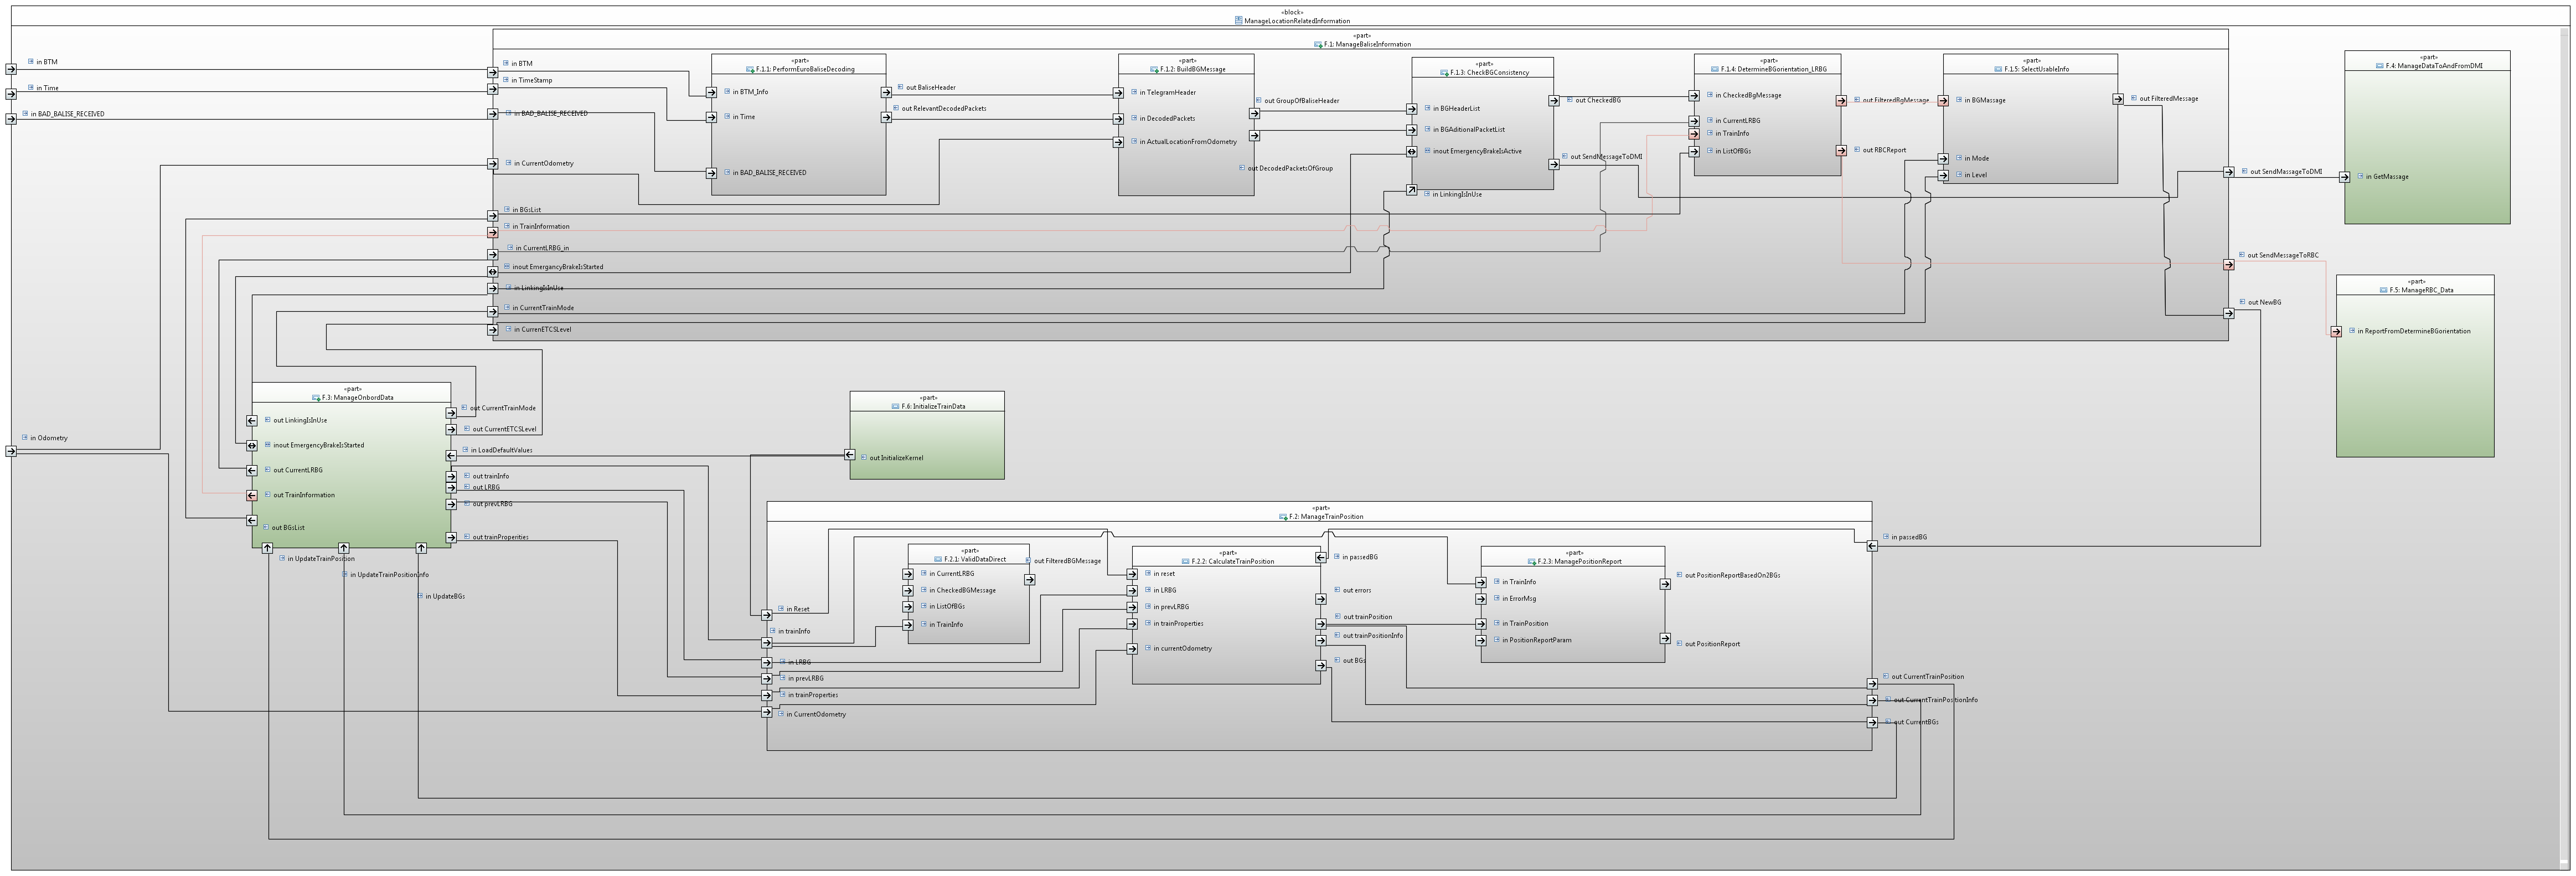
\includegraphics [angle=90, scale=0.2]{images/Current_partly_openETCS_architecture}
\caption{Centralized data structure approach architecture}
\end{figure}
 
 
 \newpage
 \subsection{centralized data structure approach}
 \begin{figure}[hbtp]
\centering
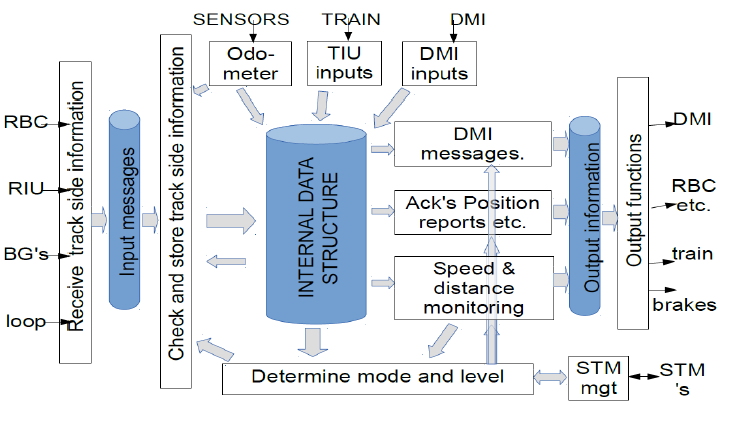
\includegraphics [scale=0.6] {images/CentralizedDataStrukture_2}
\caption{Centralized data structure approach architecture}
\end{figure}


 \begin{figure}[hbtp]
\centering
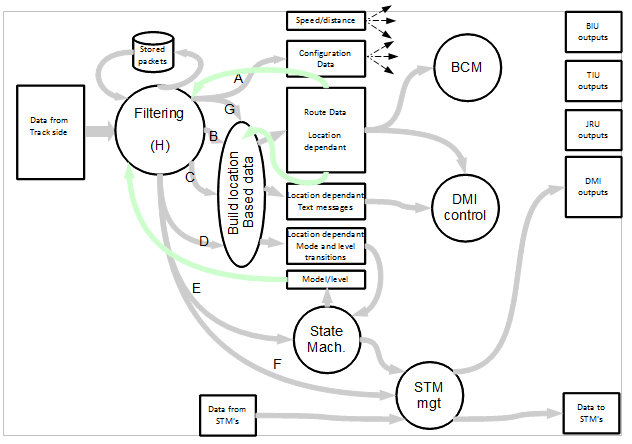
\includegraphics [scale=0.7] {images/CentralizedDataStructure_1}
\caption{Centralized data structure approach breakdown}
\end{figure}

\newpage

\subsection{Alstom High Level Approach}
 \begin{figure}[hbtp]
\section{Alstom High Level SRS Architecture}
\centering
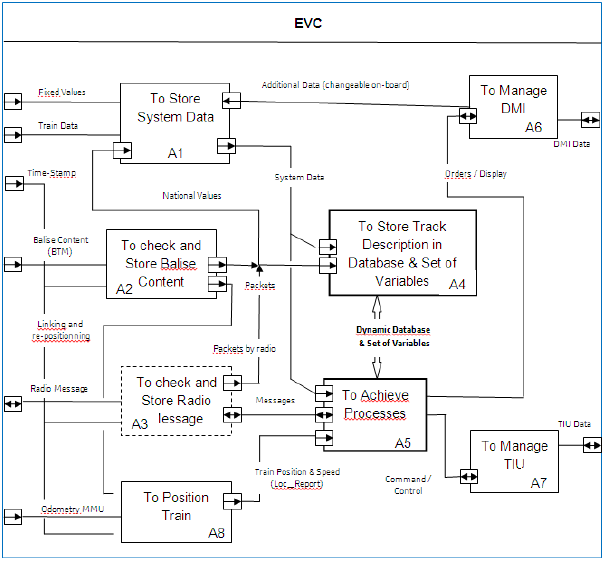
\includegraphics [scale=0.8] {images/Alstom_High_Level_Approach}
\caption{Alstom SRS Architecture Approach}
\end{figure}

\newpage
\subsection{The openETCS Tool-Chain and its impacts on the actual model}

For understanding the modelling process and the modeling guidelines, we refer to \url{https://github.com/openETCS/modeling/blob/master/DescriptionOfWork/NewModelingDescriptionOfWork.pdf}.

To summarize the design process, the following rules are in use:
\begin{itemize}
\item Papyrus / SysML is used for modelling the architecture. Functions are visible on this SysML level.
\item No behaviour model is allowed on SysML level.
\item For referencing the requirements, links from the SysML model to the requirements document (in ProR) are being used.
\item Details and especially behaviour is part of the Scade models.
\item All interfaces (see also data-dictionary below) are available on bit-level.
\item In the architecture model in SysML, all interfaces are available on a functional level for interfaces inside and outside the model and for interfaces between dedicated functions. Due to tool constrains the current model does not show all details for all interfaces (see dataDictionary).
\end{itemize}

The openETCS tool-chain for doing the modelling work consists of the following components:
\begin{itemize}
	\item [\textbf{Papyrus}]: for modelling the architecture (Kepler version).\\
	In this phase only the Kepler version of the tool can be used due to incompatibilities of the Kepler and the Luna version on the SysML model. The SysML models are stored in the following location: \url{https://github.com/openETCS/modeling/tree/master/model/sysml}.
	\item [\textbf{ProR}]: for keeping the requirements (REQIF).\\
	The subset 26 is converted into a REQIF-format and also stored in the modeling repository on Github. The openETCS toolchain supports the linking of SysML model parts to SRS-Requirements. These results are also part of the architecture.
	\item [\textbf{Scade}]: for designing and formalising the functions Scade version 15.2 is used.\\
	The models are stored in this location: \url{https://github.com/openETCS/modeling/tree/master/model/Scade}.
	With the component Scade System Scade also has a component for designing the architecture.
\end{itemize}

In principle, the synchronisation mechanism of Scade was planned to be used for synchronising the SysML architecture and the Scade models. The idea is to automatically synchronise the SysML types and blocks with the Scade type definitions and the Scade Operators. Unfortunately, with the current set of tools this idea cannot be realised. We will investigate other tools and models to find a solution. 

In addition, faults in the Kepler Papyrus version made it difficult for several members of the team to work on different submodels of the openETCS model. The issue will be solved when changing to the Luna version of Papyrus.



\section{Functions of the openETCS Model}

\subsection{openETCS Data Dictionary}

/subsubsection{dataDictionary}
%Peyman

\subsection{openETCS Generic API}


The openETCS system contains two APIs (Application Programming
Interface):
\begin{enumerate}
\item \emph{openETCS API}: the interface specification between the
EVC platform and the openETCS application;
\item \emph{model API}: the interface between the model itself written in
SCADE and the surounding run-time. Both the SCADE model and the
run-time are making the openETCS application.
\end{enumerate}

\begin{figure}[h]
\centering
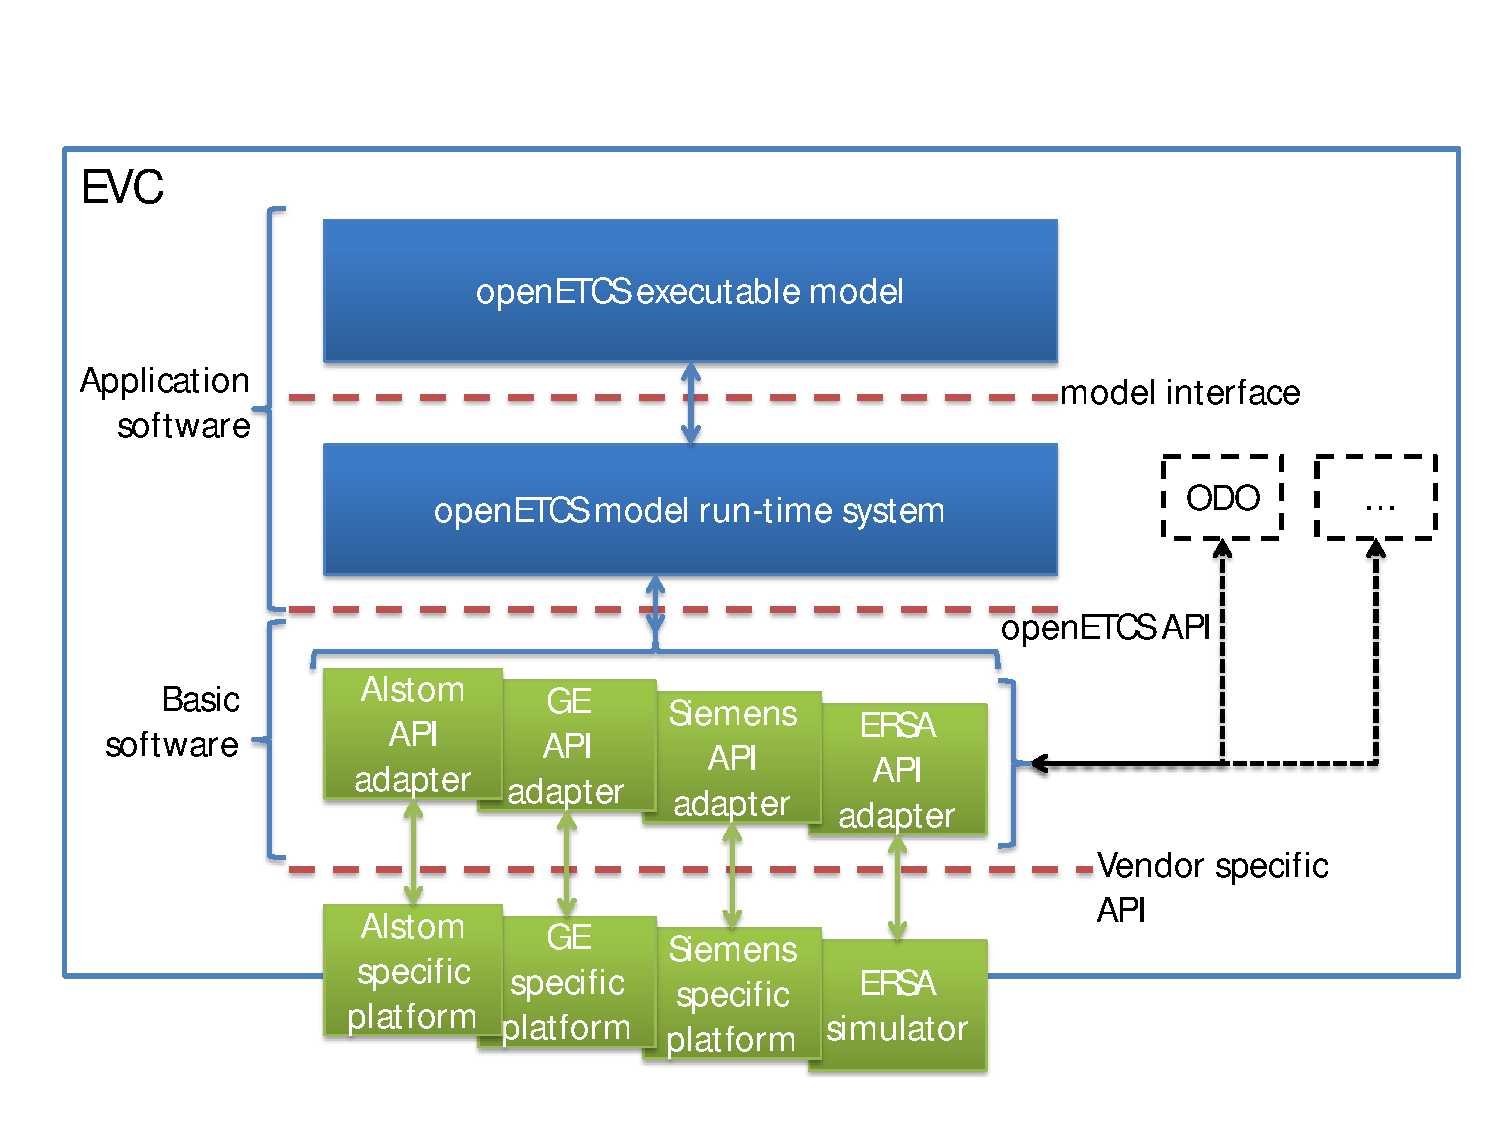
\includegraphics[width=\textwidth]{software-architecture.pdf}
\caption{openETCS software architecture}
\label{fig:software-architecture}
\end{figure}

Figure \ref{fig:software-architecture} shows both openETCS API and
model API on the software stack.

\subsubsection{openETCS API}

The openETCS API is currently defined by two documents, one written by
Alstom \cite{alstom-api} and a more abstract specification written by
openETCS members \cite{openetcs-api}.

The openETCS API defines the interfaces between the EVC platform and
the openETCS application for the following units surrounding the EVC:
\begin{itemize}
\item TIU (Train Interface Unit);
\item ODO (Odometry);
\item DMI (Driver Machine Interface);
\item STM (Specific Transmission Module, up to 8 units);
\item BTM (Balise Transmission Module);
\item LTM (Loop Transmission Module);
\item EURORADIO;
\item JRU (Juridical Recording Unit);
\item Zero or more Vendor specific unit.
\end{itemize}


\subsubsection{Model API}

The model API is currently defined by the inputs and outputs of the SCADE model.

\FIXME{How to give a precise pointer within the SCADE model? Reference
to a specific block within the model?}

For the proper working of the SCADE model, a set of assumptions are assumed:
\begin{itemize}
\item \textbf{Eurobalise (BTM)}: It is assumed that at most one
``telegram'' is provided per call of the SCADE model. This
``telegram'' is the merge of the telegrams of the balises making a
balise group.
\end{itemize}

% LocalWords:  SCADE API openETCS Alstom EVC EURORADIO Odometry balises balise


\subsection{openETCS Balise Group}


\subsubsection{Receive Eurobalise From API}
\begin{itemize}
\item \textbf{Short Description of Functionality}\\
This function defines the interface of the OBU model to the openETCS generic API for Eurobalise Messages. On the interface, either a valid telegram is provided or a telegram is indicated which could not be received correct when passing the balise. The function passes the telegram without major changes of the information to the next entity for collecting the balise group information.

%\item \textbf{{Reference to the SRS (or other requirements}\\
\item \textbf{Design Constrains and Choices}\\
\begin{enumerate}
\item Decoding of balises is done at the API. Also, packets received via the interface are already transformed into a usable shape.
\item Only packets used inside the current model are passed via the interface:\\
	Packet 5: Linking Information.\\
	Linking Information is filled into the linking array starting from index 0 without gaps. Used elements are marked as valid. Elements are sorted according to the order given by the telegram sequence.
\end{enumerate}
\end{itemize}


\subsubsection{Build BG Group}
\begin{itemize}
\item \textbf{Short Description of Functionality}\\
This entity collects telegrams received via the interface into Balise Group Information.
\item \textbf{Reference to the SRS (or other requirements}\\
\item \textbf{Design Constrains and Choices}\\
\begin{enumerate}
\item Telegrams received as invalid are passed to the ``Check-Function'' in order to process errors in communication with the trackside according to the requirements and in a single place.
Telegrams are filled into the telegram array starting from index 0 without gaps. Used elements are marked as valid. Elements are stored according to the order given by the telegram sequence. 
\item Only packets used inside the current model are passed via the interface:\\
	Packet 5: Linking Information.\\
\item In this function packets past with the telegrams is accumulated into a balise group information.\\
\item Further assumption on packet 5 (based on SRS subset 26, section 8.4.1.4)\\
(In this statement the term ``message'' is ambiguous since it can reflect to a telegram or a balise group message)
	Linking Information can only be passed once. This means, if linking information for the balise group is already collected with one of the earlier telegrams, the information will not be accumulated but overwritten.\\
\end{enumerate}
\end{itemize}

\subsubsection{Check BG Consistency}

\subsubsection{Determine BG- Orientation and LRBG}
\begin{itemize}
\item \textbf{Short Description of Functionality}\\
\item \textbf{Reference to the SRS (or other requirements}\\
\item \textbf{Design Constrains and Choices}\\
\end{itemize}
			
\subsubsection{Select Usable Info}


\subsubsection{Perform Balise Decoding}
\subsection{openETCS Train Position}

\subsubsection{F.2.2 Calculate Train Position}\label{sss:calctrainpos}

\begin{itemize}
\item \textbf{Short Description of Functionality}\\
The main purpose of the function is to calculate the locations of linked and unlinked balise groups (BGs) and the current train position while the train is running along the track. 

\begin{figure}[hbtp]
\centering
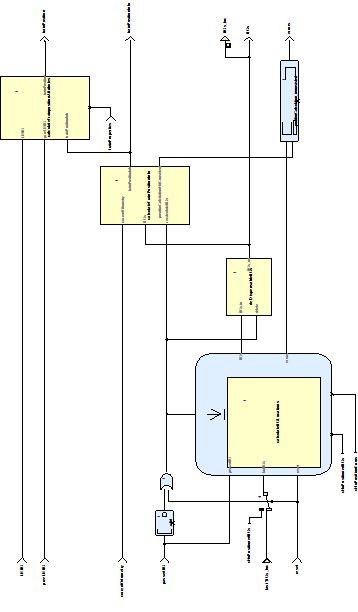
\includegraphics[scale=1]{../images/CalculateTrainPosition.png}
\caption{Structure of calculateTrainPosition}
\end{figure}


\paragraph{Functional Structure in Stages}
The whole function calculateTrainPosition is subdivided into the following steps, which are performed sequentially: 
\begin{enumerate}
\item \textbf{\textit{calculateBGLocations}}: Calculate the balise group locations\\
The first stage is triggered each time the train passes a balise group (input \textit{passedBG}). It takes the balise group header with the BG identification, the linking information (Subset 26, packet 5) and the current odometry values as inputs and calculates the location of the the passed balise group. If the passed BG has been announced via linking information previously, it takes into account the linking as well as the odometry information. If the passed BG does not meet the tolerance window announced by linking, an error flag is set. If the passed BG is an unlinked BG, its location is determined by odometry only, but related to the next previously passed linked BG, if there is one.\\
Then, if the passed BG is a linked BG comprising linking information for BGs ahead, the linking information is evaluated by creating the announced BGs and computing their locations from the linking distances.\\
The passed and the announced BGs are stored in a list \textit{BGs}, ordered by their nominal location on the track.\\
Afterwards the locations of all BGs are further improved by re-adjusting their locations with reference to the just passed BG. This optimizes the BG location inaccuries around the current train position (= location of the passed BG). 

\item \textbf{\textit{delDispensableBGs}}: Delete dispensable balise groups\\
The second stage removes balise groups supposed not to be needed any longer from the list of \textit{BGs}.\\
If the number of stored passed linked BGs exceeds the maximum number of eight as specified in subset-26-3.6.2.2.2 c), all BGs astern are deleted.
If only (passed) unlinked BGs are in the list and exceed the number of \textit{cNoOfAtLeast\_x\_unlinkedBGs}, all passed BGs astern to those are removed from the list. 

\item \textbf{\textit{calculateTrainPositionInfo}}: Calculate train position information.\\
This stage take the list of stored BGs and the current odometry values as inputs and steadily provides the current train position. 

\item \textbf{\textit{calculateTrainpositionAttributes}}: Calculate train position attribute information.\\
This stage provides several additional position related attributes that might conveniently be used by subsequent consumers in the architecture. It requires the actual LRBG and the previous LRBG to be assigned external from the list \textit{BGs}. 

\end{enumerate}

\item \textbf{Reference to the SRS (or other requirements)}\\
\\
The component calculateTrainPosition determines the location of linked and unlinked balise groups and the current train position during the train trip as specified mainly in subset-026-3.6

\item \textbf{Design Constraints and Choices}\\
\\
The following constraints and prerequisites apply:

\begin{enumerate}
\item The input data received from the balises groups must have been checked and filtered for validity, consistency and the appropriate train orientation before delivering them to calculateTrainPosition. 
\item The storage capacity for balise groups is finite. calculateTrainPosition will raise an error flag when a balise group cannot be stored due to capacity limitations.
\item calculateTrainPosition will raise an error flag if a just passed balise group is not found where announced by linking information. It will not (yet) detect when an announced balise group is missing. 
\item calculateTrainPosition is not yet prepared for train movement direction changes. 
\item calculateTrainPosition does not yet consider repositioning information.
\end{enumerate}

\end{itemize}

\subsubsection{Provide Position Report}\label{sss:provposrep}

\begin{figure}[ht]
\centering
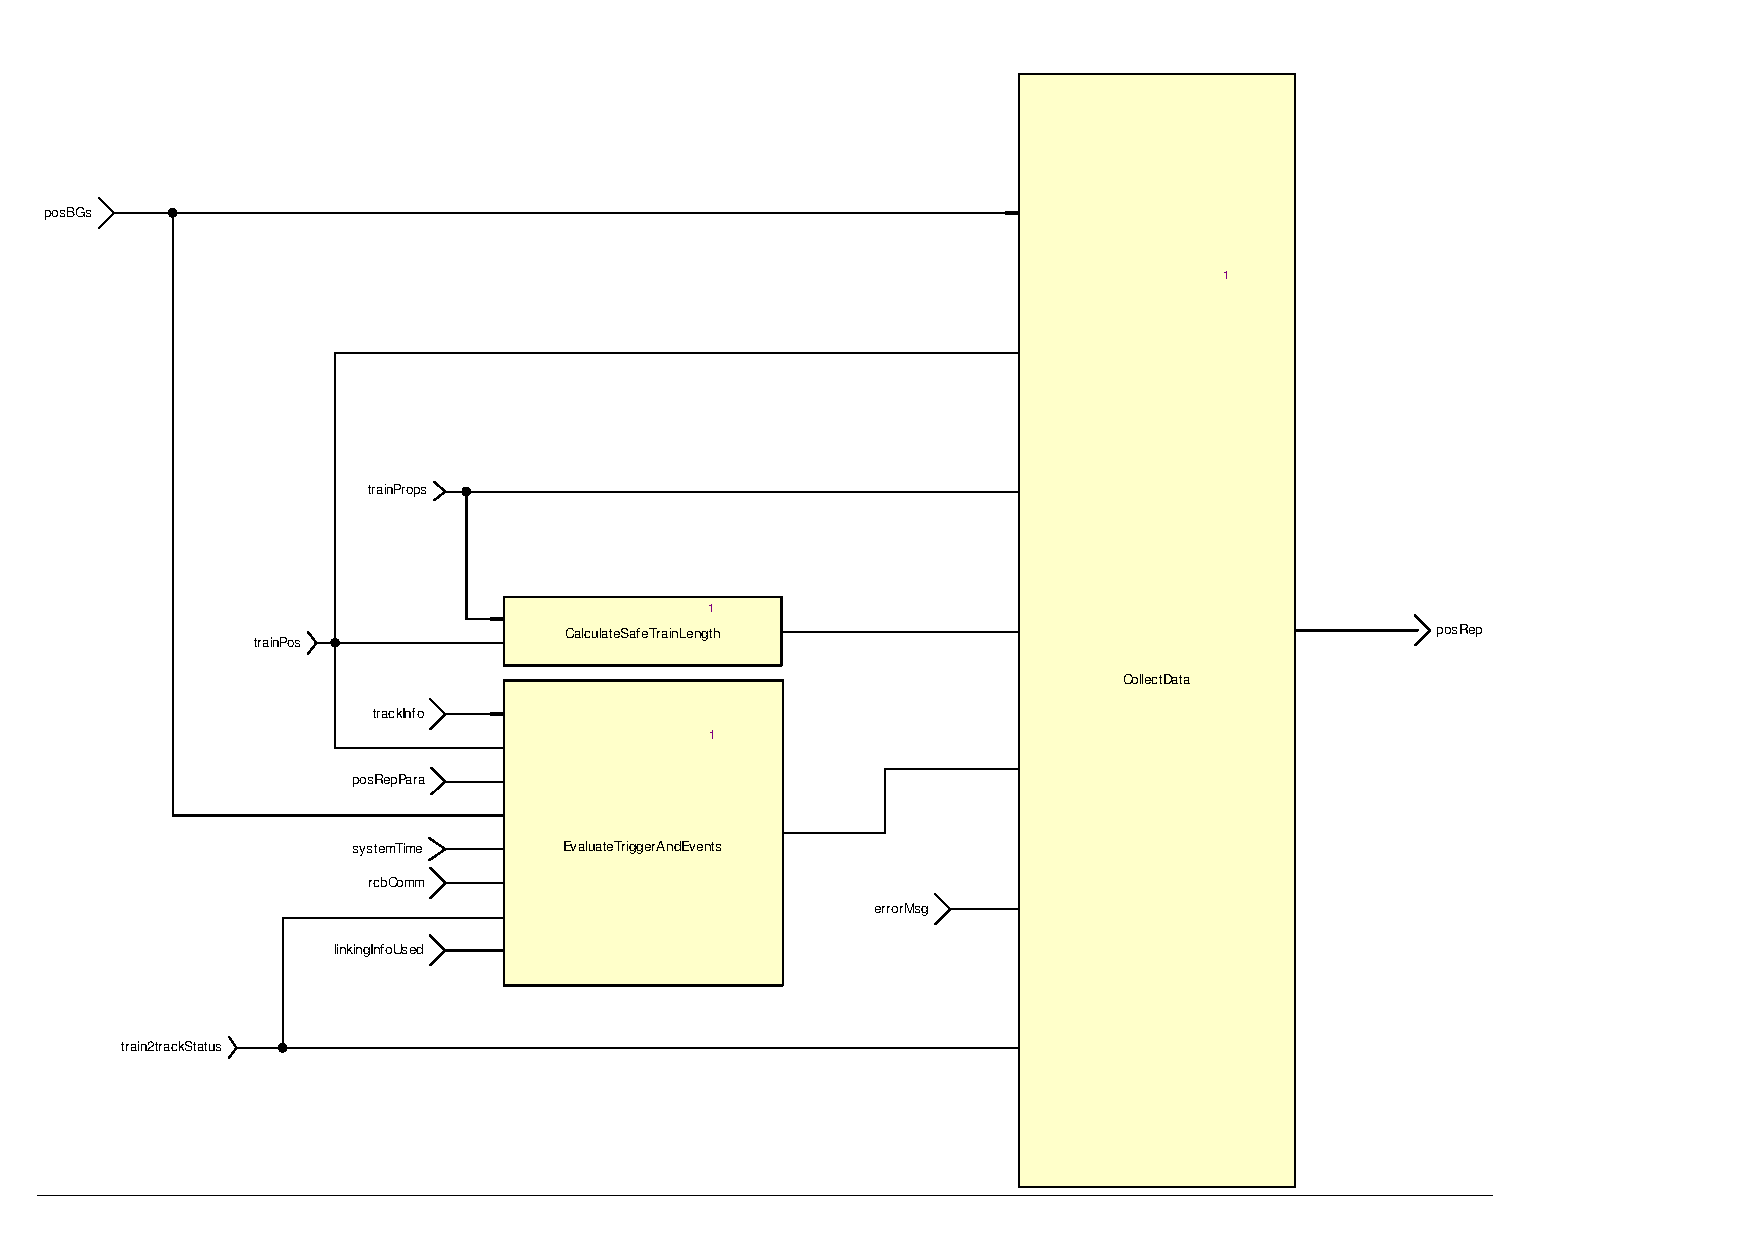
\includegraphics[scale=0.6]{../images/ProvidePositionReport.pdf}
\caption{Structure of component ProvidePositionReport}\label{fig:provideposrep}
\end{figure}

\begin{itemize}
\item \textbf{Short Description of Functionality}\\
This function takes the current train position and generates a position report which is sent to the RBC. The point in time when such a report is sent is determined from event, on the one hand, and position report parameters---which are basically triggers---provided by the RBC or a balise group passed, on the other hand. The functionality is modeled using three operations, as shown in Fig.~\ref{fig:provideposrep}, which are explained below.
\begin{description}
	\item[CalculateSafeTrainLength] Calculates the the safeTrainLength according to Chapt.~3.6.5.2.4/5.
\verb+safeTrainLength = absolute(EstimatedFrontEndPosition - MinSafeRearEnd)+, where
\verb+MinSafeRearEnd = minSafeFrontEndPosition - L_TRAIN+
	\item[EvaluateTriggerAndEvents] Returns a Boolean modeling whether the sending of the next position report is triggered or not. It is the conjunction of the evaluation of all triggers (PositionReportParameters, i.e., Packet 58) and events (see Chapt.~3.6.5.1.4).
	\item[CollectData] In this operation, data of Packet0, \dots, Packet5 and the header is aggregated to a position report.
\end{description}
\item \textbf{Reference to the SRS (or other requirements}\\
Most of the functionality is described in subset 26, chapter~3.6.5.
\item \textbf{Design Constrains and Choices}\\
\begin{enumerate}
	\item The message length (i.e., attribute \verb+L_MESSAGE+) is by default set to 0; the actual value will be set by the Bitwalker/API.
	\item The attribute \verb+Q_SCALE+ is assumed to be constant; that is, all operations using this attribute do not convert between different values of that attribute.
	\item \textit{PositionReportHeader}: The time stamp (i.e., attribute \verb+T_TRAIN+) is not set; this should be done once the message is being sent by the API
	\item \textit{Packet4}: When aggregating the data for this packet, an error message might be overwritten by a succeeding error message. Because the specification only allows to sent one error in one position report, errors are not being stored in a queue, for instance.
	\item \textit{Packet44}: This packet is currently not contained in a position report as it is not part of the kernel functions.
	\item The usage of attributes \verb+D_CYCLOC+ and \verb+T_CYCLOC+ as part of the triggers specified by the position report parameters (i.e., Packet 58 sent by the RBC) may lead to unexpected results if a big clock cycle together with small values for the attributes is used. The cause is that the current model increments at every clock cycle the reference value for the distance and time by at most \verb+D_CYCLOC+ and \verb+T_CYCLOC+, respectively and not a factor of it.
\end{enumerate}
\item \textbf{Open Issues}
\begin{enumerate}
	\item Operation \textit{EvaluateTriggerAndEvents} currently ignores parameters \verb+N_ITER+, \verb+D_LOC+ and \verb+D_LGTLOC+ which allow to specify up to 32 position at which a report has to be sent. The positions are relative to the location of a reference balise group. If the RBC sends packet 58, then it also provides a reference balise group; otherwise, if packet 58 is sent by a balise group, then this balise group serves a the reference balise group. Possible realisation in the model: Extend in the interface posRepPara (i.e., Packet 58) by a \verb+NID_BG+ referring to the reference balise group. Am assumption would be that this BG can be found in the list of passed balise group provided by \textit{CalculateTrainPosition} in Sect.~\ref{sss:calctrainpos}.
	\item The specification requires to store the last eight balise groups for which a position report has been sent (see 3.6.2.2.2.c).
	\item For all reports that contain Packet 1 (i.e., report based on two balise groups), the RBC sends a coordinate system. It is unclear where this has to be stored (i.e., somehow the balise groups have to be stored in a database which has then to be updated), see 3.4.2.3.3.6. Moreover, such a coordination system can be invalid and then has to be rejected (see 3.4.2.3.3.7-8). On a more abstract level, we need to think about the interface between the RBC and the OBU or a proper abstraction thereof.
	\item The decision whether a the report consists of packet 0 or packet 1, which is provided in 3.4.2.3.3, is currently not completely modeled. So far, 3.4.2.3.3.1 has only been modeled, thereby assuming ``the last balise group detected'' is the last balise group and not the LRBG. 3.4.2.3.3.2 is unclear. To model 3.4.2.3.3.4 I need information about the last two valid balise groups and the train running direction. This information can be obtained by adding a memory or this information will be provided by \textit{CalculateTrainPosition} in Sect.~\ref{sss:calctrainpos}. Likewise, also 3.4.2.3.3.5 requires knowledge about the last two valid balise groups.
\end{enumerate}
\end{itemize}



\nocite{*}

\bibliographystyle{unsrt}
\bibliography{erdc}



\begin{thebibliography}{9}

\bibitem{lamport94}
  Leslie Lamport,
  \emph{\LaTeX: A Document Preparation System}.
  Addison Wesley, Massachusetts,
  2nd Edition,
  1994.

\end{thebibliography}

%===================================================
%Do NOT change anything below this line

\end{document}
